\documentclass{article}
\usepackage[russian]{babel}
\usepackage[utf8]{inputenc}
\usepackage{epsfig}
\usepackage{graphicx}
\usepackage{caption}
\usepackage{subcaption}
\usepackage{amssymb}
\usepackage{amsmath}
\usepackage{bm}
\usepackage[unicode=true]{hyperref}


\DeclareMathOperator*{\argmin}{arg\,min}
\DeclareMathOperator*{\argmax}{arg\,max}
\renewcommand{\thesubsection}{} % remove subsection reference
\renewcommand{\thesubsubsection}{}

\title
    {Решение задачи MAP для марковской случайной сети}
\author
    {Новиков~А.\,В.
    \thanks{Научный руководитель: \textit{Ветров~Д.~П.}, куратор: \textit{Осокин~А.}}
    \\МГУ, ВМиК, каф. ММП
    }

\begin{document}
\maketitle

\pagebreak
\setcounter{tocdepth}{1}
 \tableofcontents
\pagebreak

\section{Введение}
Марковские случайные поля (MRF) --- это популярный подход к решению задач анализа данных. Чаще всего их используют в компьютерном зрении, где область применения простирается от устранения шума и сегментации изображений до стерео--реконструкции, распознавания образов и редактирования изображений.
Одна из самых важных задач, возникающих при использовании MRF --- максимизация апостериорной вероятности~(MAP)~\cite{ApplicationAndComp}. Для большинства приложений задача MAP является NP--трудной.\\

В данной работе проводится обзор и сравнение существующих state--of--the--art подходов к решению этой задачи.

% \subsection{Вклад}
% Платформа для сравнения алгоритмов и выводы о перспективности тех или иных способов оптимизации.



\section{Данные}
Чтобы получить воспроизводимые результаты мы использовали данные, опубликованные в работе~\cite{Alahari}. Это задачи стерео--реконструкции с MRF типа решетка и парными потенциала Поттса. В них количество переменных равно количеству пикселей на изображениях, а количество меток $K$ соответствует разрешению по оси Z у восстановленной карты глубины. В наших экспериментах участвовали следующие стерео--пары:
\begin{center}
    \begin{tabular}{ | l | l | l |}
    \hline
    Название & Количество переменных & Количество меток\\ \hline
    Tsukuba  & 110592 & 16\\ \hline
    Venus  & 166222 & 20\\ \hline
    Cones  & 168750 & 60\\ \hline
    \end{tabular}
\end{center}


\section{Обозначения}
Марковская случайная сеть задана графом $G = (V, E)$. Переменные прямой задачи обозначаются $x_a \in \{1, \dots, K\}$ и индексируются вершиной $a \in V$. $X = \{x_a\}_{a \in V}$. Двойственная функция обозначается как $f(\Lambda)$. $\mathcal{L}$ --- это множество ограничений на $\Lambda$, а $g^k$ --- проекция субградиента $f(\Lambda)$ на множество $\mathcal{L}$ (на $k$--ой итерации).\\
$P_C(\cdot)$ используется для обозначения Евклидовой проекции на множество~$C$ (т.~е. $P_C(x_0) = \argmin_{x \in C} \left \| x - x_0 \right \|_2$).

\section{Постановка задачи}
На MRF заданной графом $G = (V, E)$ ставится задача максимизации апостериорной вероятности:
\begin{equation*}
    P(x~|~z) \propto \prod_{a \in V} \psi (z_a~|~x_a) \prod_{(a,b) \in E} \psi_{ab} (x_{a}, x_{b}) \rightarrow \max_{X}
\end{equation*}
От неё переходят к задаче минимизации минус логарифма вероятности, который называют \textit{энергией}:
\begin{equation}
    E(x) = \sum_{a \in V} \varphi_a (x_a) + \sum_{(a,b) \in E} \varphi_{ab} (x_{a}, x_{b}) \rightarrow \min_{X}
    \label{eq:orig_problem}
\end{equation}
Унарный потенциал $\varphi_a (p)$ отражает стоимость присваивания $x_a = p$, а парный потенциал $\varphi_{ab} (p, q)$~--- стоимость присваивания $x_{a} = p, x_{b} = q$.\\
В общем случае~(\ref{eq:orig_problem}) --- NP--трудная задача дискретной оптимизации, но существует частные случаи для которых она решается эффективно~\cite{belief_propagation}.

\section{Обзор методов}
Одним из хорошо зарекомендовавших себя подходов к решению данной задачи считается применение методов основанных на совершении шагов (например $\alpha$--расширение)~\cite{NewComparison}.
Мы будем сравнивать $\alpha$--расширение с TRW--S~\cite{TRWS} и методами основанными на
двойственном разложении, в которых задача минимизации
исходной энергии сводится к максимизации
двойственной энергии (это функция в отличие от исходной энергии
является вогнутой и кусочно--линейной).
Алгоритмы этой группы отличает конкретный метод максимизации.

Полный список методов участвующих в сравнении:
\begin{itemize}
\item $\alpha$--расширение\footnote{http://www.csd.uwo.ca/faculty/olga/software.html}~\cite{AlphaExp}~\cite{AlphaExp2}~\cite{AlphaExp3}
\item TRW--S\footnote{http://pub.ist.ac.at/~vnk/papers/TRW-S.html}~\cite{TRWS}
\item Субградиентный подъём~\cite{Subgradient}
\item Методы на основе \textit{пучков}~(bundle methods)~\cite{Bundle}
\item L--BFGS
% \item <<Полная декомпозиция>>
\end{itemize}

\section{Двойственное разложение}
Заменим каждую $K$--значную переменную $x_a$ на набор бинарных переменных $\{y_{a,1} \dots y_{a,K} \}$: $y_{a,p} = 1 \Leftrightarrow x_a = p$. Аналогично для каждого ребра графа $(a,b) \in E$ введем бинарные переменные $y_{ab,11}, y_{ab,12}\dots, y_{ab,KK}$: $y_{ab,pq} = 1 \Leftrightarrow x_a = p, x_b = q$. Обозначим $\theta_{a,p} = \varphi_{a} (p)$, $\theta_{ab,pq} = \varphi_{ab} (p, q)$.\\
В новых обозначениях энергия становится линейной функцией:
\begin{equation}
  E(Y, \Theta) = \sum_{a \in V} \sum_{p = 1}^{K} \theta_{a,p} y_{a,p} + \sum_{(a,b) \in E} \sum_{p,q = 1,1}^{K} \theta_{ab,pq} y_{ab,pq} \rightarrow \min_{Y \in \mathcal{M}}
\label{eq:main_problem}
\end{equation}
\begin{align*}
  \mathcal{M} = \Bigg \{ Y~|~&y_{a,p}, y_{ab,pq} \in \{0,~1\}, \sum_{p = 1}^{K} y_{a,p} = 1,\\
&\sum_{p = 1}^{K} y_{ab,pq} = y_{b,q}, \sum_{q = 1}^{K} y_{ab,pq} = y_{a,p} \Bigg \}
\end{align*}

Заменим множество ограничений $\mathcal{M}$ на более широкое $\mathcal{R}$~(данный прием называется LP--релаксацей):
\begin{align*}
  \mathcal{R} = \Bigg \{ Y~|~&y_{a,p}, y_{ab,pq} \in \hm{[} \mathbf{ 0,~1} \hm{]}, \sum_{p = 1}^{K} y_{a,p} = 1,\\
&\sum_{p = 1}^{K} y_{ab,pq} = y_{b,q}, \sum_{q = 1}^{K} y_{ab,pq} = y_{a,p} \Bigg \}
\end{align*}
Мы получаем оценку снизу:
\begin{equation}
\min_{y \in \mathcal{M}} E(Y, \Theta) \geq \min_{Y \in \mathcal{R}} E(Y, \Theta).
\label{eq:relaxation}
\end{equation}
Если граф G является деревом,~--- в~(\ref{eq:relaxation}) достигается равенство.

Разобьем граф на деревья $\{D^t\}_{t=1}^T$ так, чтобы каждая вершина и каждое ребро G входили ходя бы в одно дерево. Обозначим за $n_a$ число деревьев, включающих вершину $a$.
\begin{equation*}
\theta_{a,p}^t = \left\{ 
\begin{array}{l l}
\frac{\theta_{a,p}}{n_a}, & a \in D^t\\
0, & a \not \in D^t
\end{array} \right.
\end{equation*}
Аналогично, $n_{ab}$ --- число деревьев включающих ребро $(a, b)$,
\begin{equation*}
\theta_{ab,pq}^t = \left\{ 
\begin{array}{l l}
\frac{\theta_{ab,pq}}{n_{ab}}, & (a,b) \in D^t\\
0, & (a,b) \not \in D^t
\end{array} \right.
\end{equation*}

Таким образом, для каждого дерева $D^t$ мы определили массив переменных $\Theta^t$, причем
\begin{equation*}
\Theta = \sum_{t = 1}^{T} \Theta^t,
\end{equation*}
\begin{equation*}
E(Y, \Theta) = \sum_{t = 1}^{T} E(Y, \Theta^t).
\end{equation*}

Введем дополнительные переменные $\Lambda = \{\Lambda^t\}_{t=1}^T = \{\{\lambda_{a,p}^t\},\{\lambda_{ab,pq}^t\}\}_{t=1}^T \in \mathcal{L}$, где $\mathcal{L}$ задается ограничениями:
\begin{equation*}
\sum_{t = 1}^{T} \lambda_{a,p}^t = 0, \forall a, p,
\end{equation*}
\begin{equation*}
\sum_{t = 1}^{T} \lambda_{ab,pq}^t = 0, \forall (a, b), p,q.
\end{equation*}

Собирая всё вместе:
\begin{align*}
&\min_{Y \in \mathcal{M}} E(Y~|~\Theta) \geq \min_{Y \in \mathcal{R}} E(Y~|~\Theta) = \\
&= \min_{Y \in \mathcal{R}} E(Y~|~\Theta) + \sum_{t = 1}^{T} \left [ \sum_{a \in V} \sum_{p = 1}^{K} \lambda_{a,p}^t y_{a,p} + \sum_{(a,b) \in E} \sum_{p,q = 1}^{K} \lambda_{ab,pq}^t y_{ab,pq} \right] = \\
&=\min_{Y \in \mathcal{R}} E(Y~|~\Theta + \Lambda) \geq \sum_{t = 1}^{T} \min_{Y \in \mathcal{R}} E(Y~|~\Theta^t + \Lambda^t)
\end{align*}
В каждом слагаемом у нас LP--релаксация задачи~(\ref{eq:main_problem}) для дерева, а значит:
\begin{equation}
\sum_{t = 1}^{T} \min_{Y \in \mathcal{R}} E(Y~|~\Theta^t + \Lambda^t) = \sum_{t = 1}^{T} \min_{Y \in \mathcal{M}} E(Y~|~\Theta^t + \Lambda^t) = f(\Lambda),
\end{equation}
где $f(\Lambda)$ называют \textit{двойственной функцией}.\\

Заметим, что $\min_{Y \in \mathcal{M}} E(Y~|~\Theta^t + \Lambda^t)$ является минимум конечного (хотя и очень большого) числа линейных по $\Lambda^t$ функций, т.~е. вогнутой функцией.

Для применения методов максимизации функции $f(\Lambda)$ нам понадобятся проекции её субградиентов на множество $\mathcal{L}$:\\
\begin{equation}
P_{\mathcal{L}} \left( \frac{\partial}{\partial \lambda_{a,p}^t} f(\Lambda) \right ) = \widehat{y}_{a,p}^t - \frac{\sum_{\{t' | a \in D^{t'}\}} \widehat{y}_{a,p}^{t'}}{n_a}
\end{equation}
, где $\widehat{y}_{ap}^t = arg\min_{Y \in \mathcal{M}} E(Y~|~\Theta^t + \Lambda^t)$, то есть решение внутренней задачи минимизации на дереве. Аналогично,
\begin{equation}
P_{\mathcal{L}} \left( \frac{\partial}{\partial \lambda_{ab,pq}^t} f(\Lambda) \right ) = \widehat{y}_{ab,pq}^t - \frac{\sum_{\{t' | (a,b) \in D^{t'}\}} \widehat{y}_{ab,pq}^{t'}}{n_{ab}}
\end{equation}
, где $\widehat{y}_{ab,pq}^t = arg\min_{Y \in \mathcal{M}} E(Y~|~\Theta^t + \Lambda^t)$.

\section{Методы оптимизации двойственной функции}
На шаге $k$ обозначим за $g^k$ проекцию субградиента $f(\Lambda^k)$:
\begin{equation}
g^k = P_{\mathcal{L}} \left( \frac{\partial}{\partial \Lambda} f(\Lambda) \right ) \bigg|_{\Lambda = \Lambda^k}
\end{equation}

\subsection{Субградиентный подъём}
В основе метода субградиентного подъёма лежит идея на каждом шаге идти в сторону проекции субградиента $f(\Lambda)$:
\begin{equation}
\Lambda^{k+1} = \Lambda^k + \alpha^k \cdot g^k
\end{equation}
Результаты работы данного метода зависят от выбора
последовательности шагов $\alpha^k$.
Мы использовали константный, адаптивный шаг, неточную
одномерную оптимизацию по величине шага, а так же
точную одномерную оптимизацию.\\

Как и ожидалось, субградиентный подъём с константным шагом сходится плохо~(рис.~\ref{fig:constant_subgradient}).\\
\begin{figure}
    \centering
    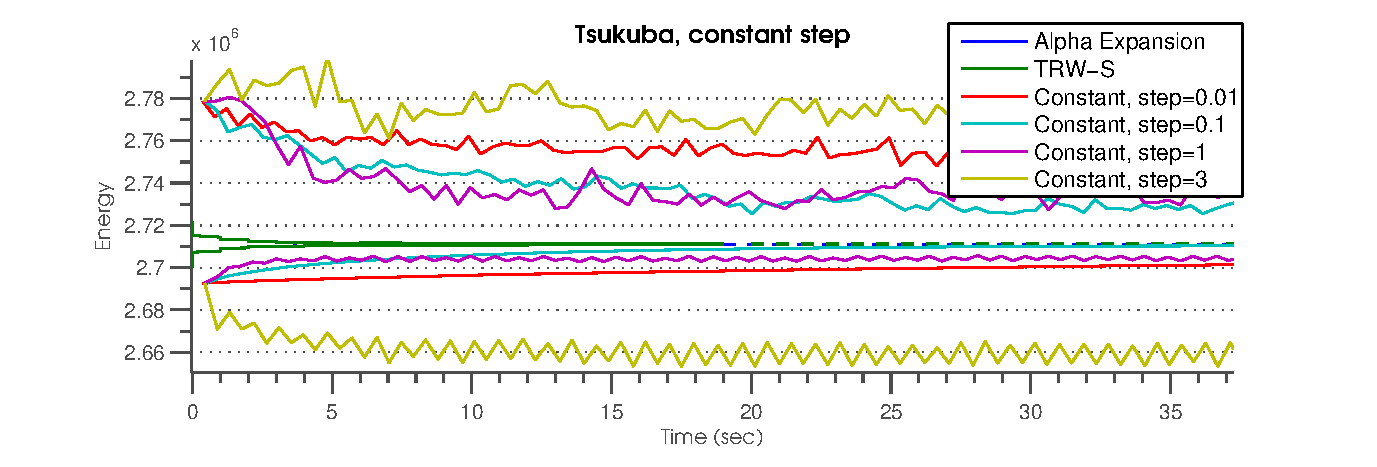
\includegraphics[width=\textwidth]{constant_subgradient_tsukuba.eps}
    \caption{Субградиентный подъём с константным шагом для различных констант.}
    \label{fig:constant_subgradient}
\end{figure}
В случае адаптивного шага использовалась формула предложенная Комодакисом~\cite{SubgradientWeights}:\\
\begin{equation}
\alpha^k = \frac{Approx^k - Dual^k}{\left \| g^k \right \|^2}
\end{equation}
$Dual^k$~--- это текущее значение двойственной функции, а $Approx^k$~--- оценка оптимума двойственной функции, вычисляемая по формуле:\\
$Approx^k = BestDual^k + \delta^k$,\\
$BestDual^k = \max_{t \in \{1 \dots k\}} f(\Lambda^t)$~--- это лучшее на данный момент значение двойственной функции,\\
\begin{equation}
    \delta^{k+1} = \begin{cases}
    \gamma_0 \delta^k, & Dual^k > Dual^{k-1},\\
    max(\gamma_1 \delta^k, \epsilon) & Dual^k \leqslant  Dual^{k-1}.
    \end{cases}
\end{equation}
\begin{figure}
    \centering
    \begin{subfigure}[t]{\textwidth}
            \centering
            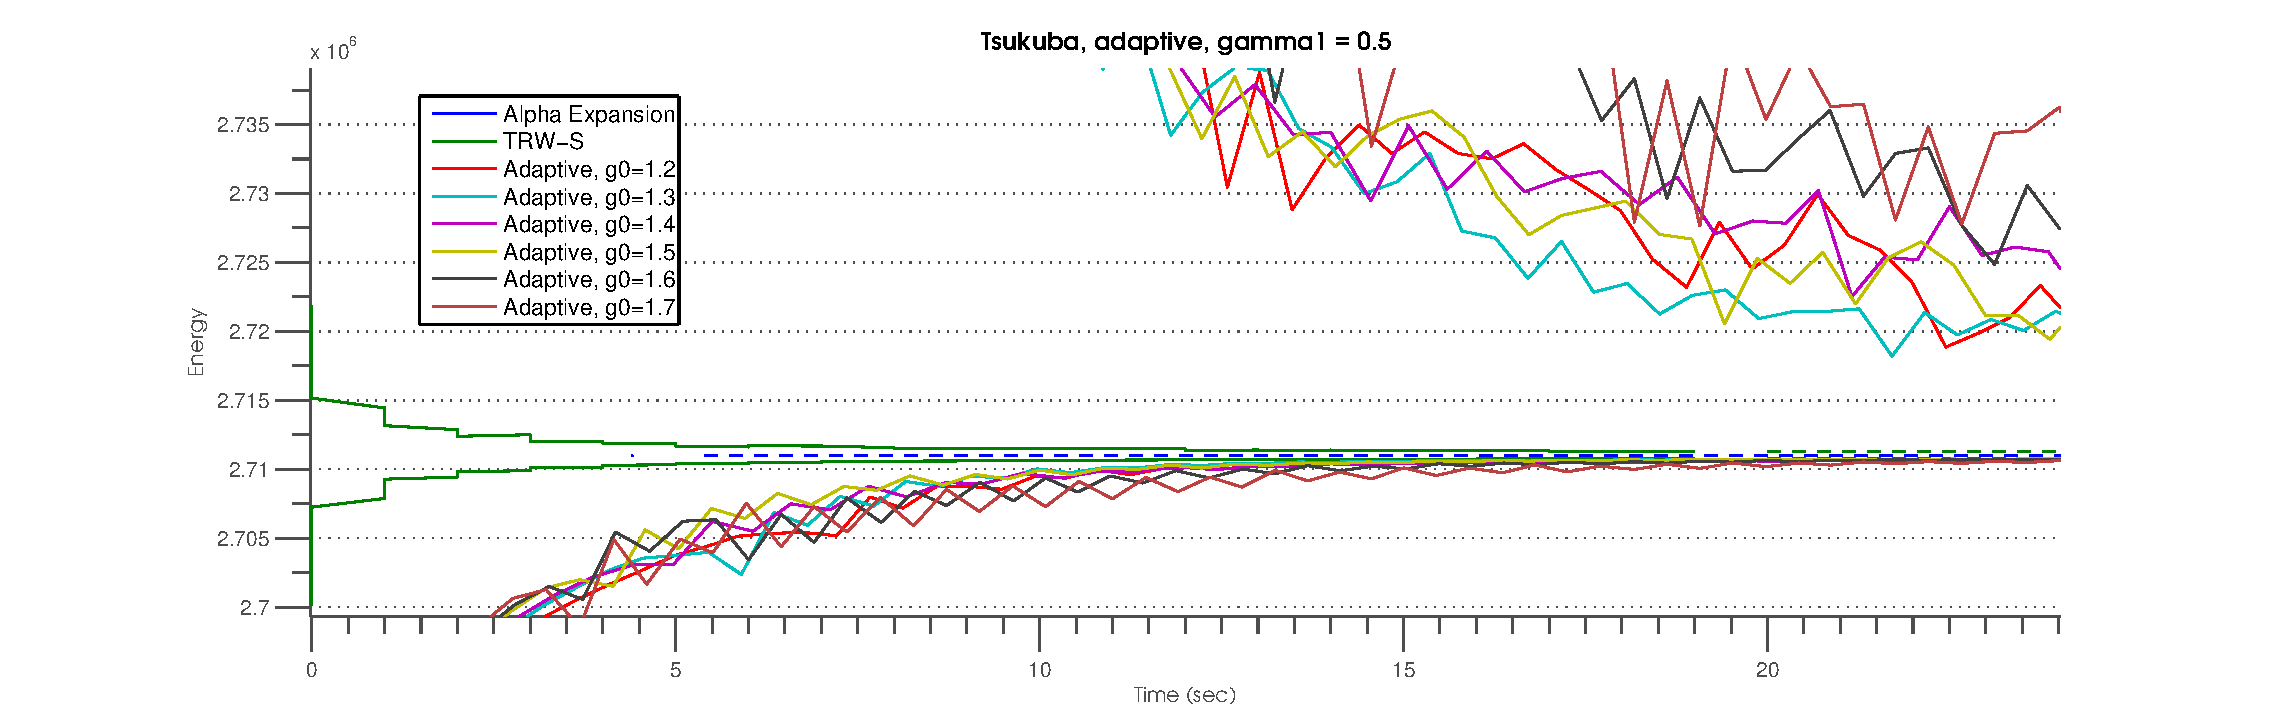
\includegraphics[width=\textwidth]{adaptive_g0_tsukuba}
            \caption{Стерео--пара tsukuba.}
    \end{subfigure}
    \begin{subfigure}[t]{\textwidth}
            \centering
            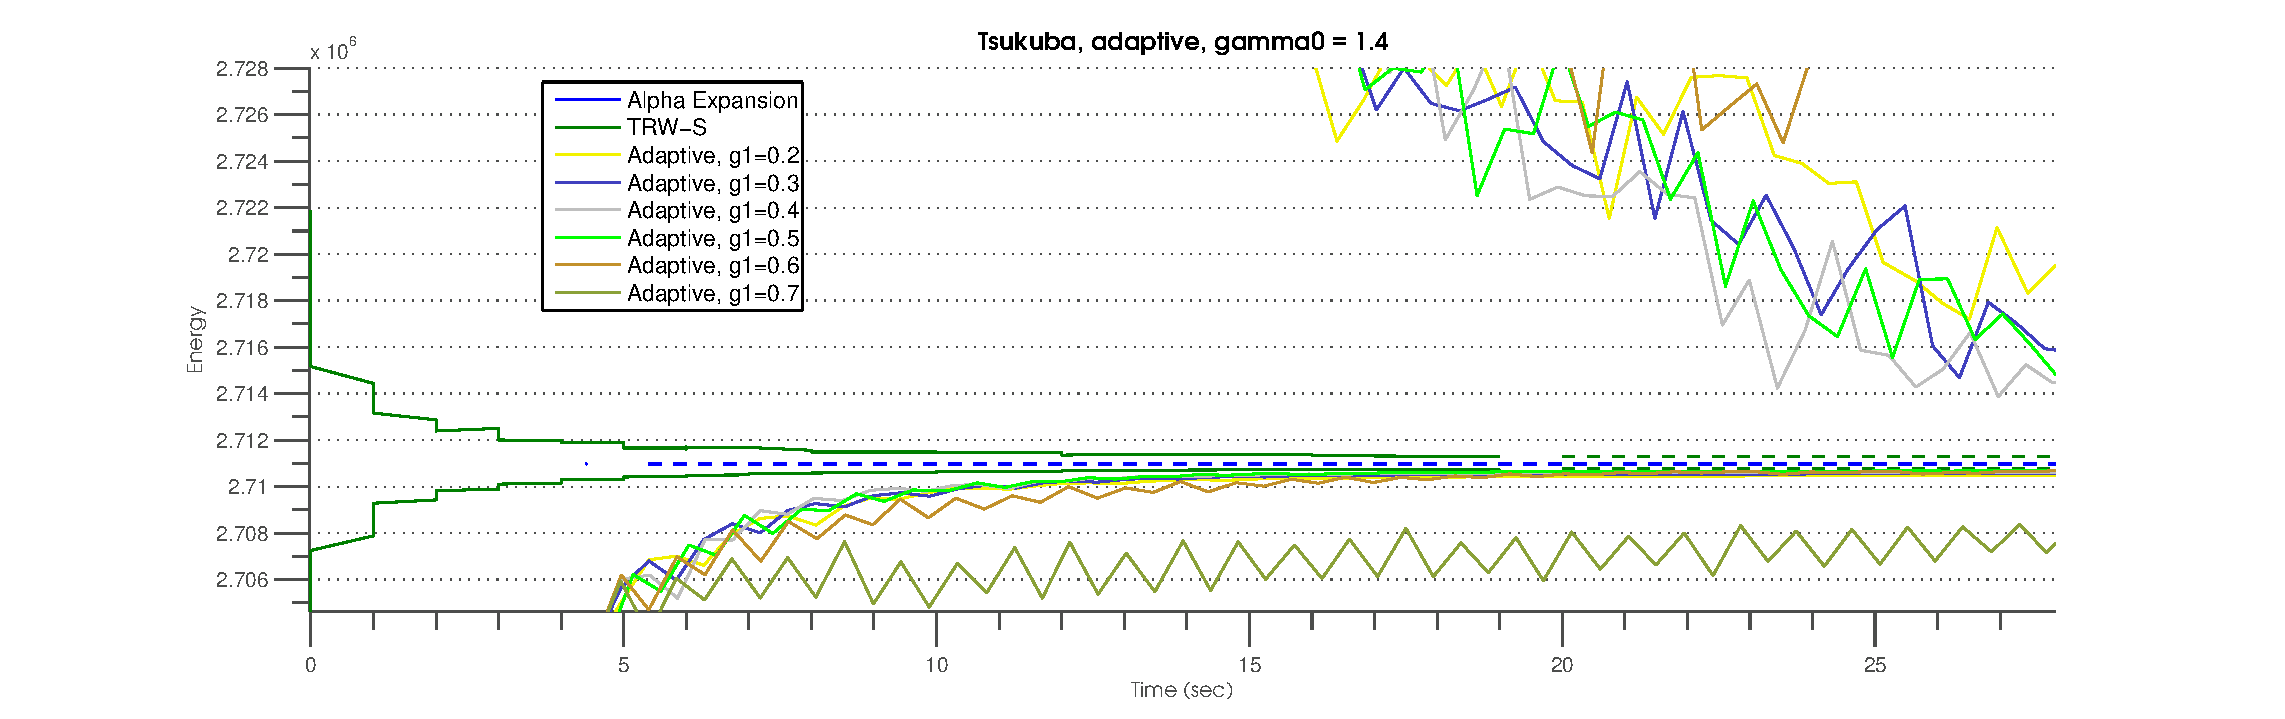
\includegraphics[width=\textwidth]{adaptive_g1_tsukuba}
    \end{subfigure}
    \caption{Подбор параметров адаптивного субградиетного подъёма.}
    \label{fig:adaptive_params}
\end{figure}

$\gamma_0$, $\gamma_1$, $\epsilon$~--- параметры метода, выбранные нами эмпирически~(рис.~\ref{fig:adaptive_params},~\ref{fig:adaptive_params_extra}).\\
$\gamma_0 = 1.4$\\
$\gamma_1 = 0.5$\\
$\epsilon^k = \frac{1}{k}$\\


\subsubsection{Одномерная оптимизация}
\begin{figure}
    \centering
    \begin{subfigure}[t]{\textwidth}
            \centering
            \includegraphics[width=0.9\textwidth]{profile_subgradient_tsukuba}
    \end{subfigure}
    \begin{subfigure}[t]{\textwidth}
            \centering
            \includegraphics[width=0.9\textwidth]{profile_subgradient_cones}
    \end{subfigure}
    \caption{Профиль двойственной функции вдоль направления оптимизации и неточные максимумы найденные различными алгоритмами.}
    \label{fig:profile}
\end{figure}

\begin{figure}
    \centering
    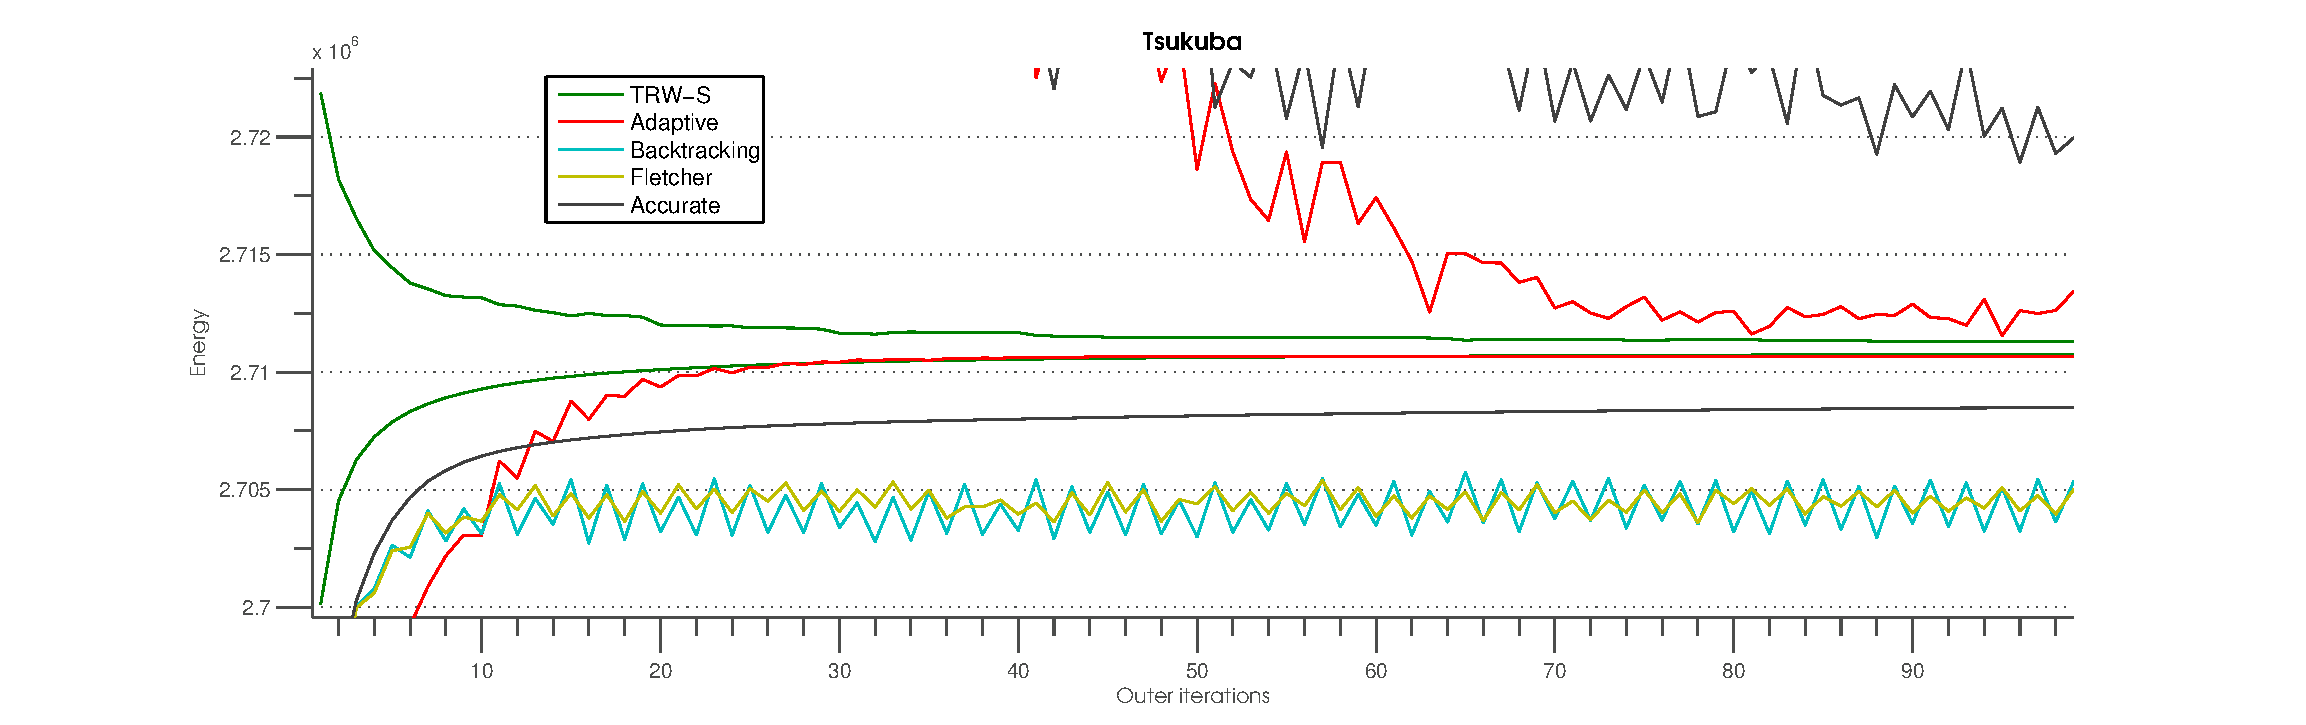
\includegraphics[width=\textwidth]{subgradient_tsukuba}
    \caption{Субградиентный подъём с разными схемами выбора шага. На горизонтальной оси отложены внешние итерации метода, то есть время потраченное на одномерную оптимизацию не учитывается.}
    \label{fig:1d_optimization}
\end{figure}
Несмотря на то, что профиль\footnote{профилем функции мы будем называть график значения функции вдоль определенного направления.} двойственной функции является кусочно линейным, он очень близок к гладкому~(рис.~\ref{fig:profile}), так что методы неточной одномерной оптимизации кажутся довольно перспективным направлением работы (мы верим, что данную задачу почти гладкой выпуклой одномерной оптимизации можно решить эффективно). Нами были опробованы метод Флетчера и <<backtracking>>~\cite{1d_optimization}.\\
Тем не менее мы выяснили что одномерная оптимизация не приносит ожидаемой пользы~(рис.~\ref{fig:1d_optimization}, видно что даже если использовать точную оптимизацию и не учитывать потраченное на неё время, результат получается хуже чем при использовании адаптивного подхода).


\subsection{Методы на основе \textit{пучков}~(<<bundle methods>>)}
Основная идея методов этого класса --- ограничить двойственную функцию $f(\Lambda)$ сверху с помощью вогнутой кусочно--линейной функции $\hat{f}(\Lambda)$ и дальше оптимизировать (уточняя на каждом шаге) именно $\hat{f}(\Lambda)$. Эта функция строится по последовательности точек $\{\Lambda^k\}$, значений в этих точках $\{f(\Lambda^k)\}$ и субградиентов $g^k \in \partial f(\Lambda^k)$ так, что $f(\Lambda) \leq \hat{f}(\Lambda)$ и $f(\Lambda^k) = \hat{f}(\Lambda^k)$. Вместе $\{\Lambda^k\}$, $\{f(\Lambda^k)\}$ и  $g^k \in \partial f(\Lambda^k)$ составляют \textit{пучок} $\mathcal{B}$.
\begin{equation}
\hat{f}(\Lambda) = \min_{(\Lambda{}', f(\Lambda{}'), g{}') \in \mathcal{B}} \{f(\Lambda{}') + <g{}', \Lambda - \Lambda{}'>\}
\end{equation}

Для генерации последовательности точек мы используем проксимальный алгоритм:\\
\begin{equation}
\Lambda^{k + 1} = \argmax_{\Lambda} \{\hat{f}(\Lambda)  - \frac{w^k}{2} \left \| \Lambda - \overline{\Lambda} \right \|_2^2\}
\label{eq:bundle_update}
\end{equation}
где $w^k > 0$ нужен чтобы удержать $\Lambda^{k + 1}$ около текущего кандидата на решение ($\overline{\Lambda}$), где $\hat{f}(\Lambda)$ близок к $f(\Lambda)$. По смыслу данный параметр соответствует величине обратной длине шага --- чем он больше, тем ближе новая точка будет к исходной.\\
Если новая точка $\Lambda^{k + 1}$ не ведет к значительному прогрессу, мы не меняем текущую оценку решения $\overline{\Lambda}$, а только уточняем $\hat{f}(\Lambda)$ добавляя в пучок $(\Lambda^{k+1}, f(\Lambda^{k+1}), g^{k+1})$. $k$--ый шаг в таком случае называют \textit{нулевым шагом}. В противном случае мы обновляем $\overline{\Lambda} = \Lambda^{k + 1}$, это называется \textit{значительным шагом}. Чтобы понять какой вид шага нужно выполнять сейчас, мы сравниваем увеличение $f(\Lambda^{k+1})$ и $\hat{f}(\Lambda^{k+1})$ относительно $f(\overline{\Lambda})$. Если отношение этих величин больше чем заранее зафиксированный параметр $m_L$, тогда аппроксимация $\hat{f}(\Lambda)$ достаточно точна чтобы предпринять значительный шаг.\\

Задача~(\ref{eq:bundle_update}) может быть сведена к квадратичному программированию размерности равной количеству элементов в пучке~\cite{Bundle}.\\

В описанном алгоритме осталось два аспекта сильно влияющих на итоговую скорость оптимизации --- это управление размером пучка $\mathcal{B}$ (пучок должен быть достаточно маленьким чтобы можно было быстро решать задачу квадратичного программирования возникающую на каждой итерации) и выбор последовательности весов $\{w^k\}$.

\subsubsection{Управление размером пучка}
Чтобы ограничить размер пучка есть два основных подхода~\cite{Bundle}:\\
\begin{itemize}
\item Удалять самое малонарушаемое ограничение ограничение как только размер пучка превысит некоторой фиксированный порог $n$. Метод гарантированно сойдётся если выбрать $n$ достаточно большим, но к сожалению достаточное $n$ сравнимо с размерностью двойственного пространства (в нашем случае порядка миллионов). Тем не менее даже с небольшим размером $n$ методы успешно работают на практике~\cite{Bundle}, хотя для них нельзя гарантировать сходимость.\\
\item Другой подход предложен Kiwiel~\cite{ABundle}. Он предлагает заменить весь пучок одним \emph{агрегированным субградиентом} (выпуклой комбинацией всех субградиентов виденных до сих пор) без потерь теоретических гарантий.
\end{itemize}


\subsubsection{Последовательность весов}
\begin{figure}[t]
  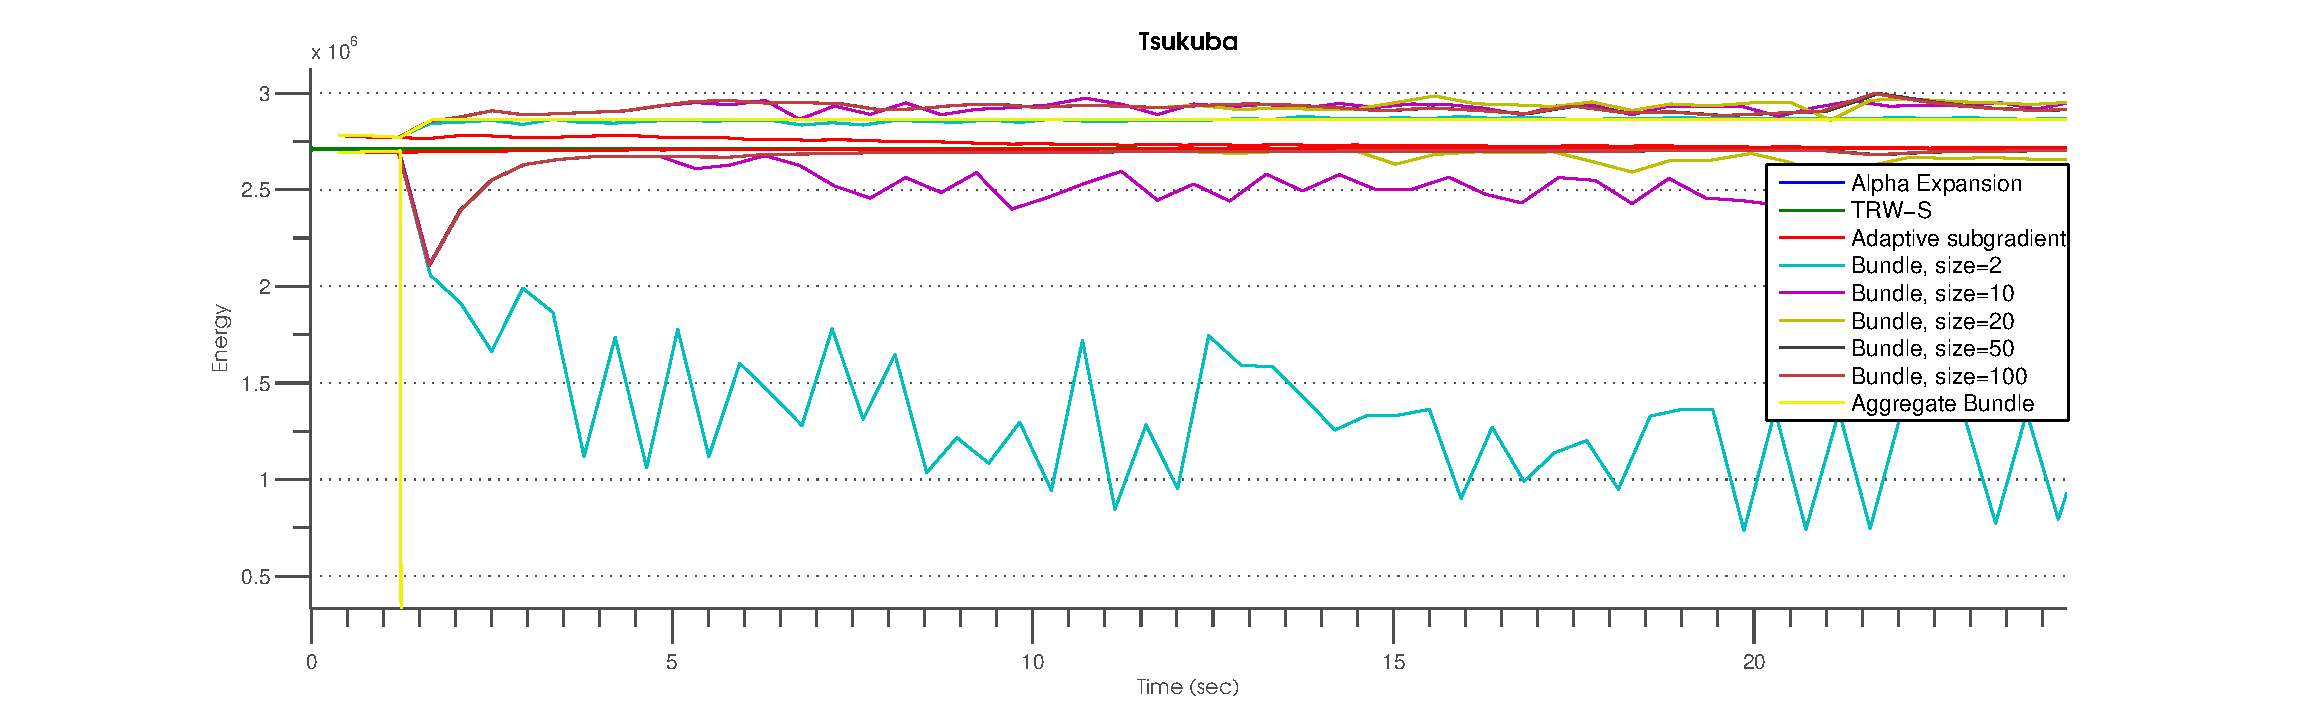
\includegraphics[width=1.1\textwidth]{bundle_weights_problem_tsukuba.eps}
  \caption{Использование предложенной схемы выбора весов~(\ref{eq:bundle_weights}) ведет к расхождению и метода пучка и метода агрегированного пучка.}
  \label{fig:bundle_weights_problem}
\end{figure}

\begin{figure}[t]
  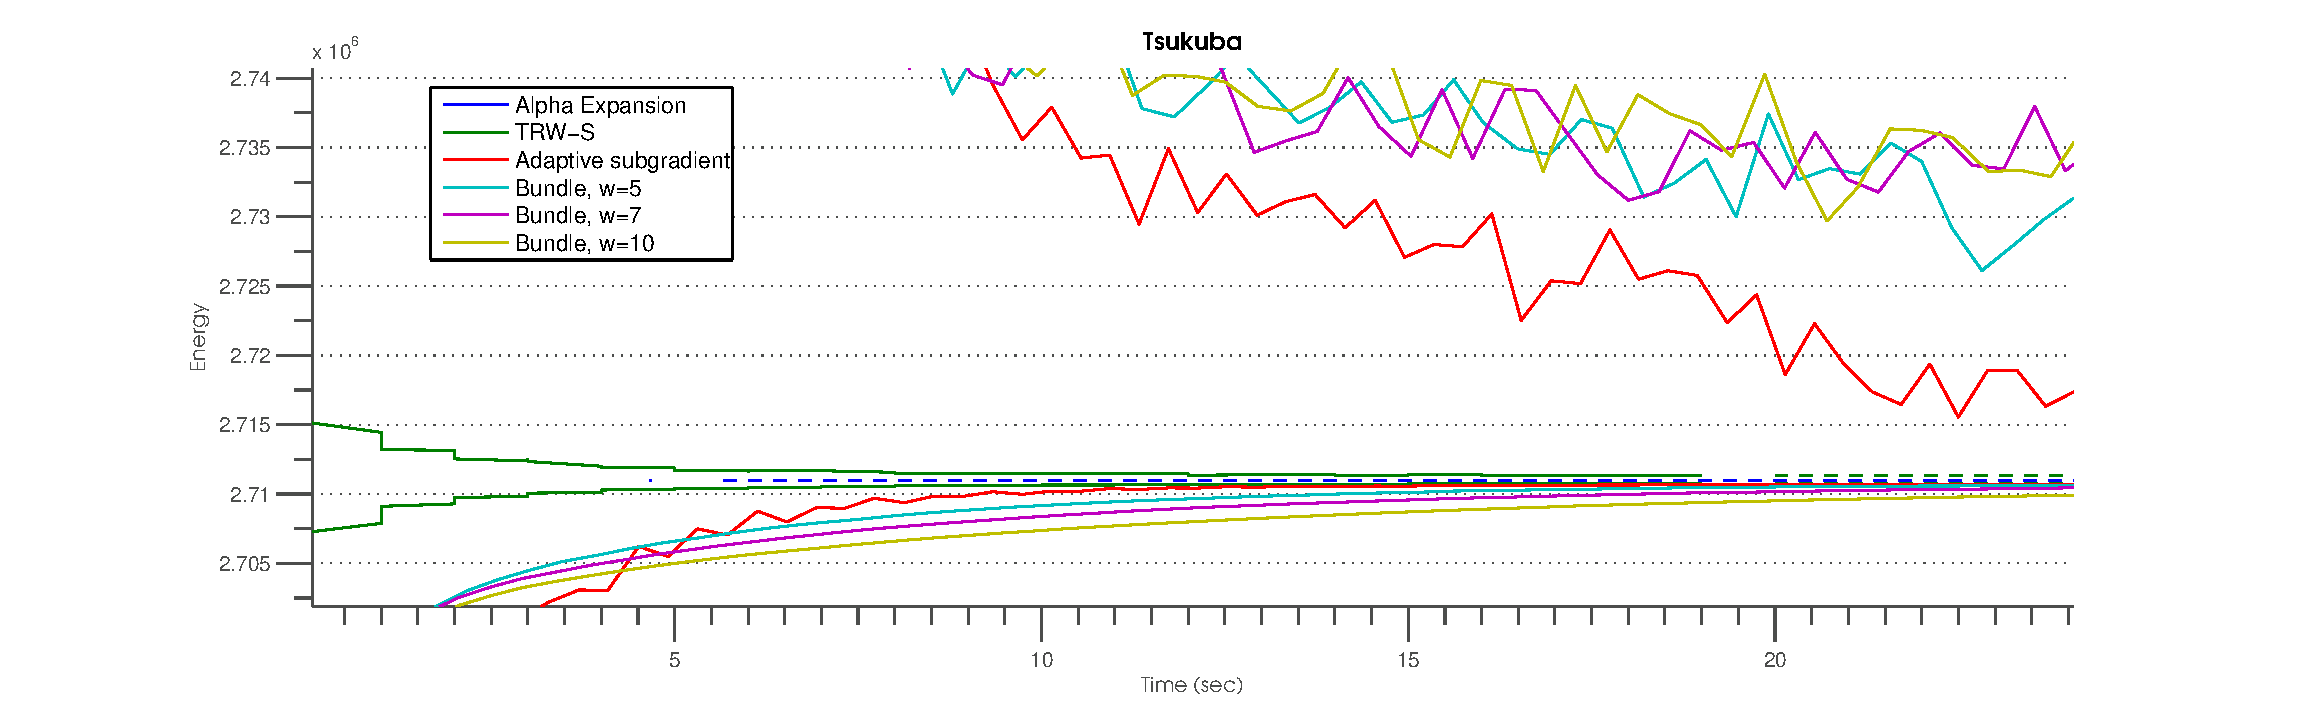
\includegraphics[width=1.1\textwidth]{bundle_const_weight_tsukuba.eps}
  \caption{Метод пучка с различными константными весами.}
  \label{fig:bundle_const_weight}
\end{figure}

Для выбора весов авторы подхода предлагают следующую схему:\\
\begin{equation}
   w^k = P_{[w_\text{min}, w_\text{max}]} \left ( \left (\gamma \cdot \frac{\min_{t \in \{1 \dots k\}}Upper^t - \max_{t \in \{1 \dots k\}} Dual^t}{\left \| g^k \right \|} \right )^{-1}\right )
   \label{eq:bundle_weights}
\end{equation}
и добиваются значительных успехов~\cite{Bundle}. Хотя мы использовали те же данные и параметры алгоритмов для тестирования, методы на основе пучков с таким выбором весов расходится~(рис.~\ref{fig:bundle_weights_problem}). Схема~(\ref{eq:bundle_weights}) на всех протестированных стерео--парах выбирает веса порядка $0.01$. Если же отказаться от схемы~(\ref{eq:bundle_weights}) и положить вес равным большой константе, метод работает хуже чем у авторов подхода, но с разумным качеством~(рис.~\ref{fig:bundle_const_weight},~\ref{fig:bundle_const_weight_extra}). На данном этапе мы будем использовать $w^k = 5$ для метода пучка и $w^k = 1$ для метода агрегированного пучка, но в будущем рассчитываем разобраться с проблемой выбора весов и отказаться от примитивного подхода.

\subsection{L--BFGS}
Мы использовали реализацию L--BFGS из библиотеки HANSO\footnote{http://www.cs.nyu.edu/overton/software/hanso/} (версия для негладкой оптимизации) и применяли её для максимизации двойственной функции.

\section{Сравнение подходов}
\begin{figure}
    \centering
    \begin{subfigure}[t]{\textwidth}
            \centering
            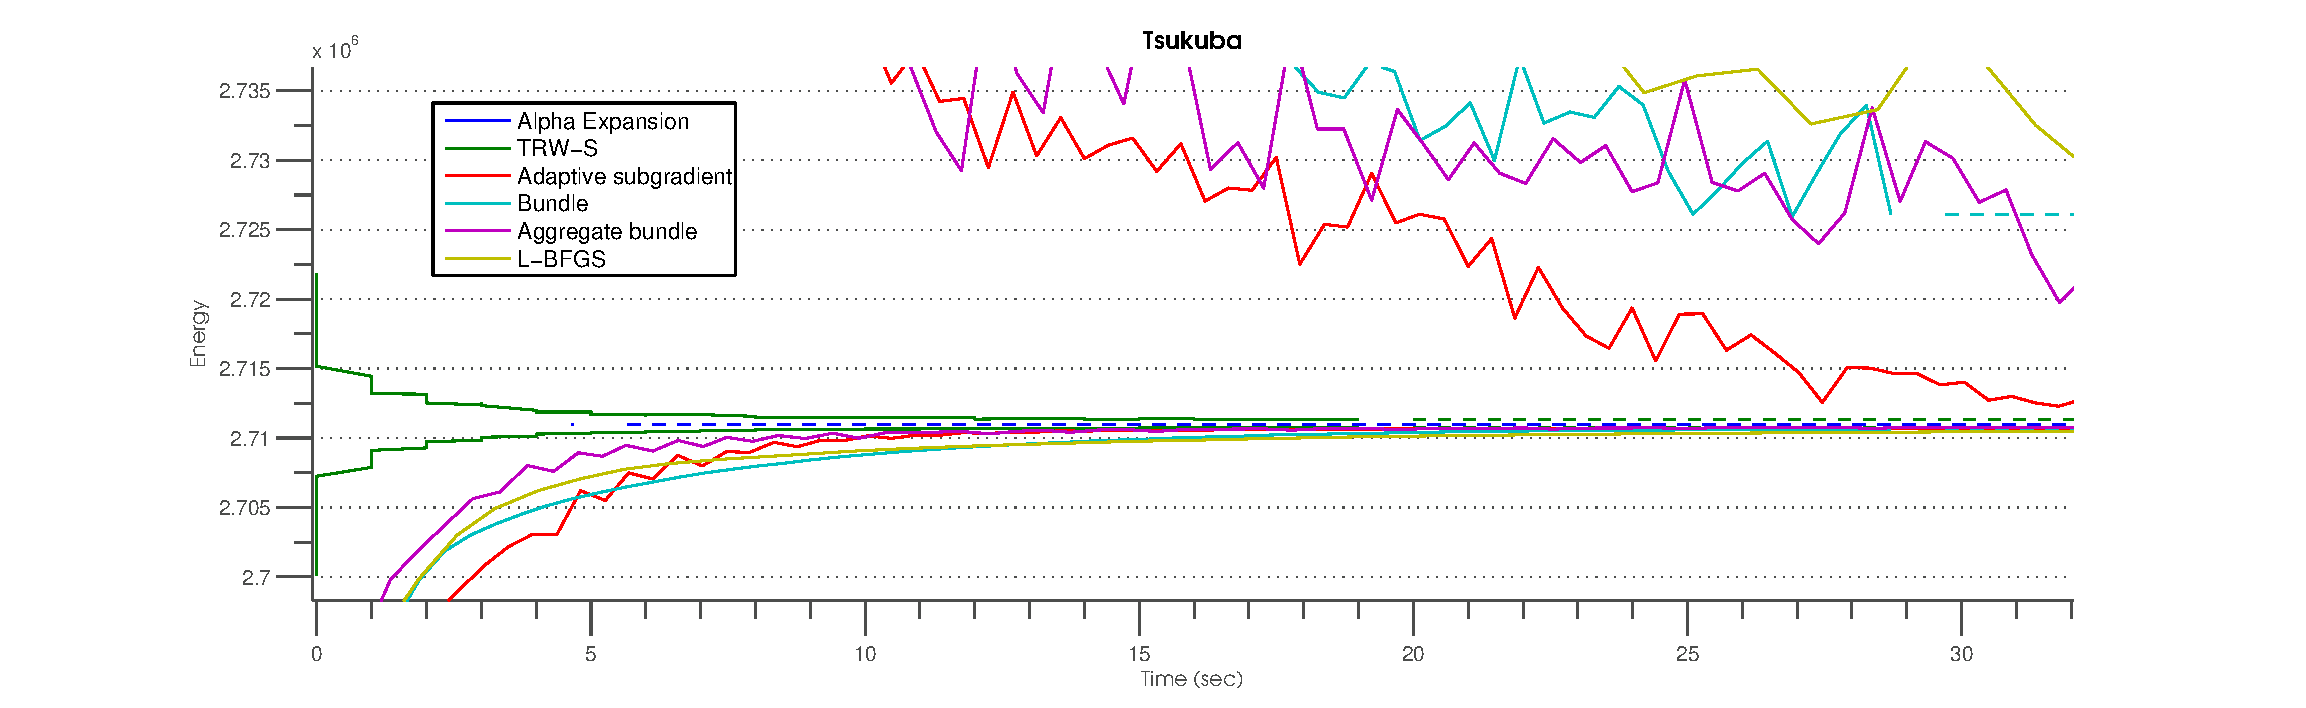
\includegraphics[width=0.9\textwidth]{comparative_small_tsukuba.eps}
    \end{subfigure}
    \begin{subfigure}[t]{\textwidth}
            \centering
            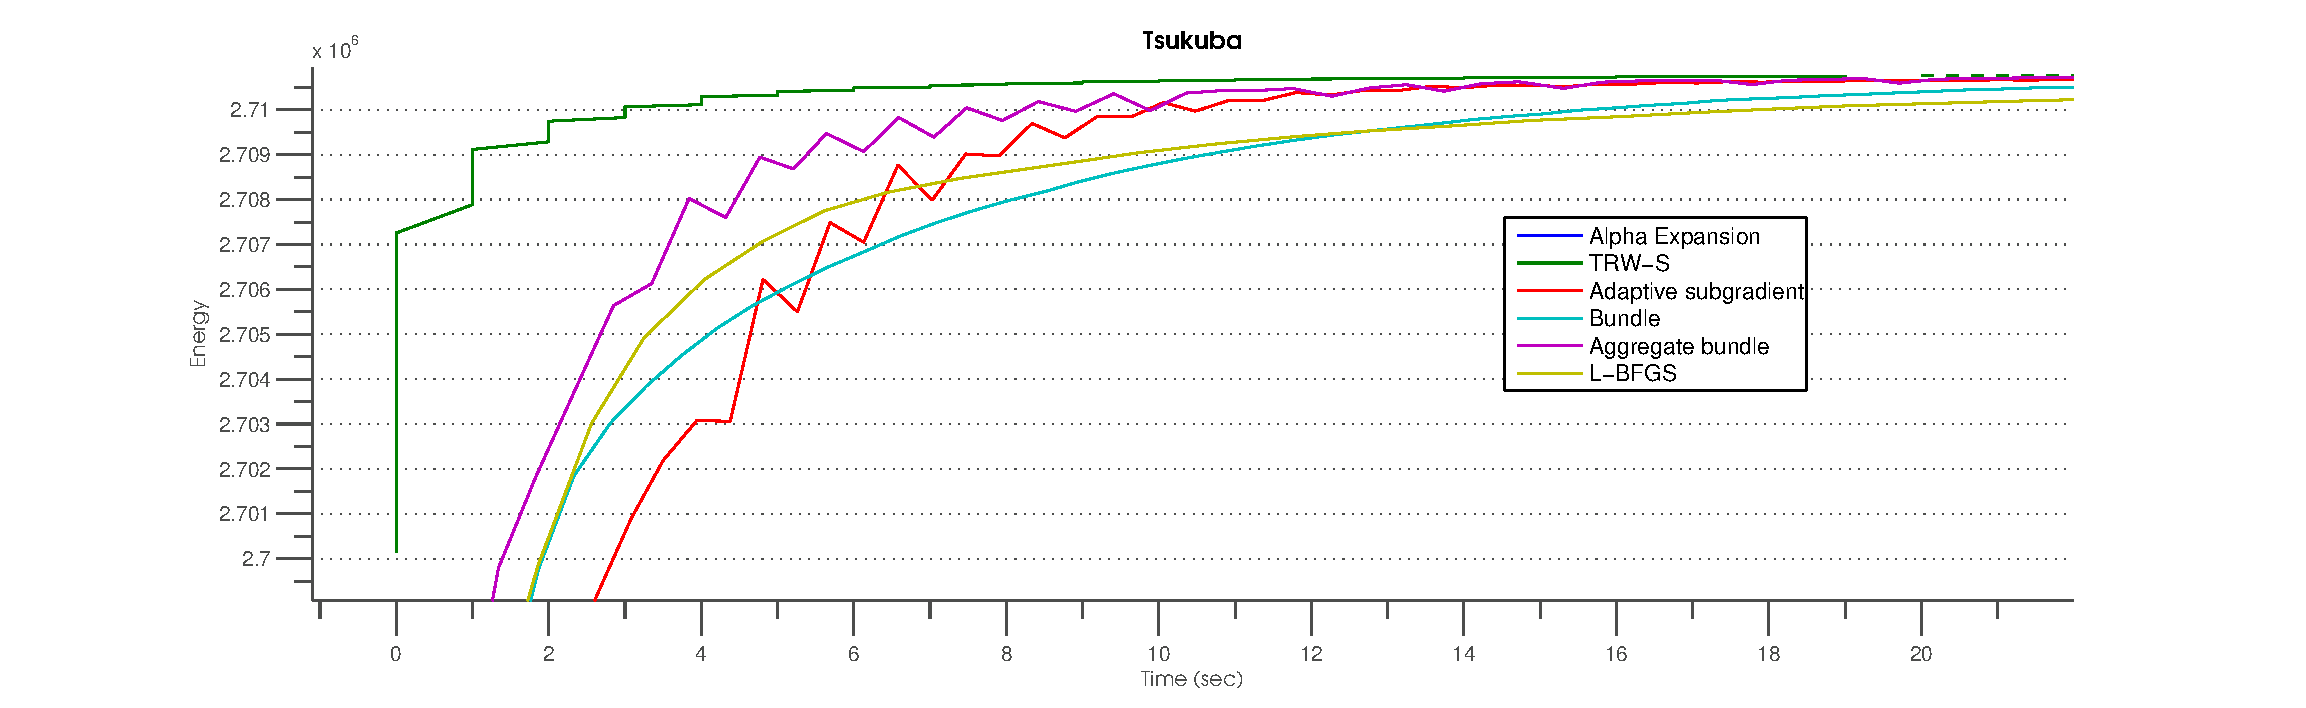
\includegraphics[width=0.9\textwidth]{comparative_tsukuba.eps}
    \end{subfigure}
    \caption{Итоговое сравнение алгоритмов оптимизации энергии.}
    \label{fig:comparative}
\end{figure}
В наших экспериментах~(рис.~\ref{fig:comparative},~\ref{fig:comparative_extra}) лучше всего работает метод агрегированного пучка (несмотря на константный выбор веса $w^k = 1$). Неожиданно неплохо работает метод адаптивного субградиентного подъёма.

\section{Выводы, вклад}
Нами был реализован фреймоворк для удобного сравнивания алгоритмов оптимизации двойственной энергии (исходные коды и примеры использования есть в открытом доступе\footnote{https://github.com/AlexHomework/TRW}). С его помощью были выявлены перспективные направления для дальнейшей работы и показано, что метод субградиентного подъёма работает на уровне подходов на основе пучков и применения метода L--BFGS.

\section{Приложение}
В этом разделе приведены дополнительные графики, иллюстрирующие тезисы на большем числе примеров.
\begin{figure}
    \centering
    \begin{subfigure}[t]{\textwidth}
            \centering
            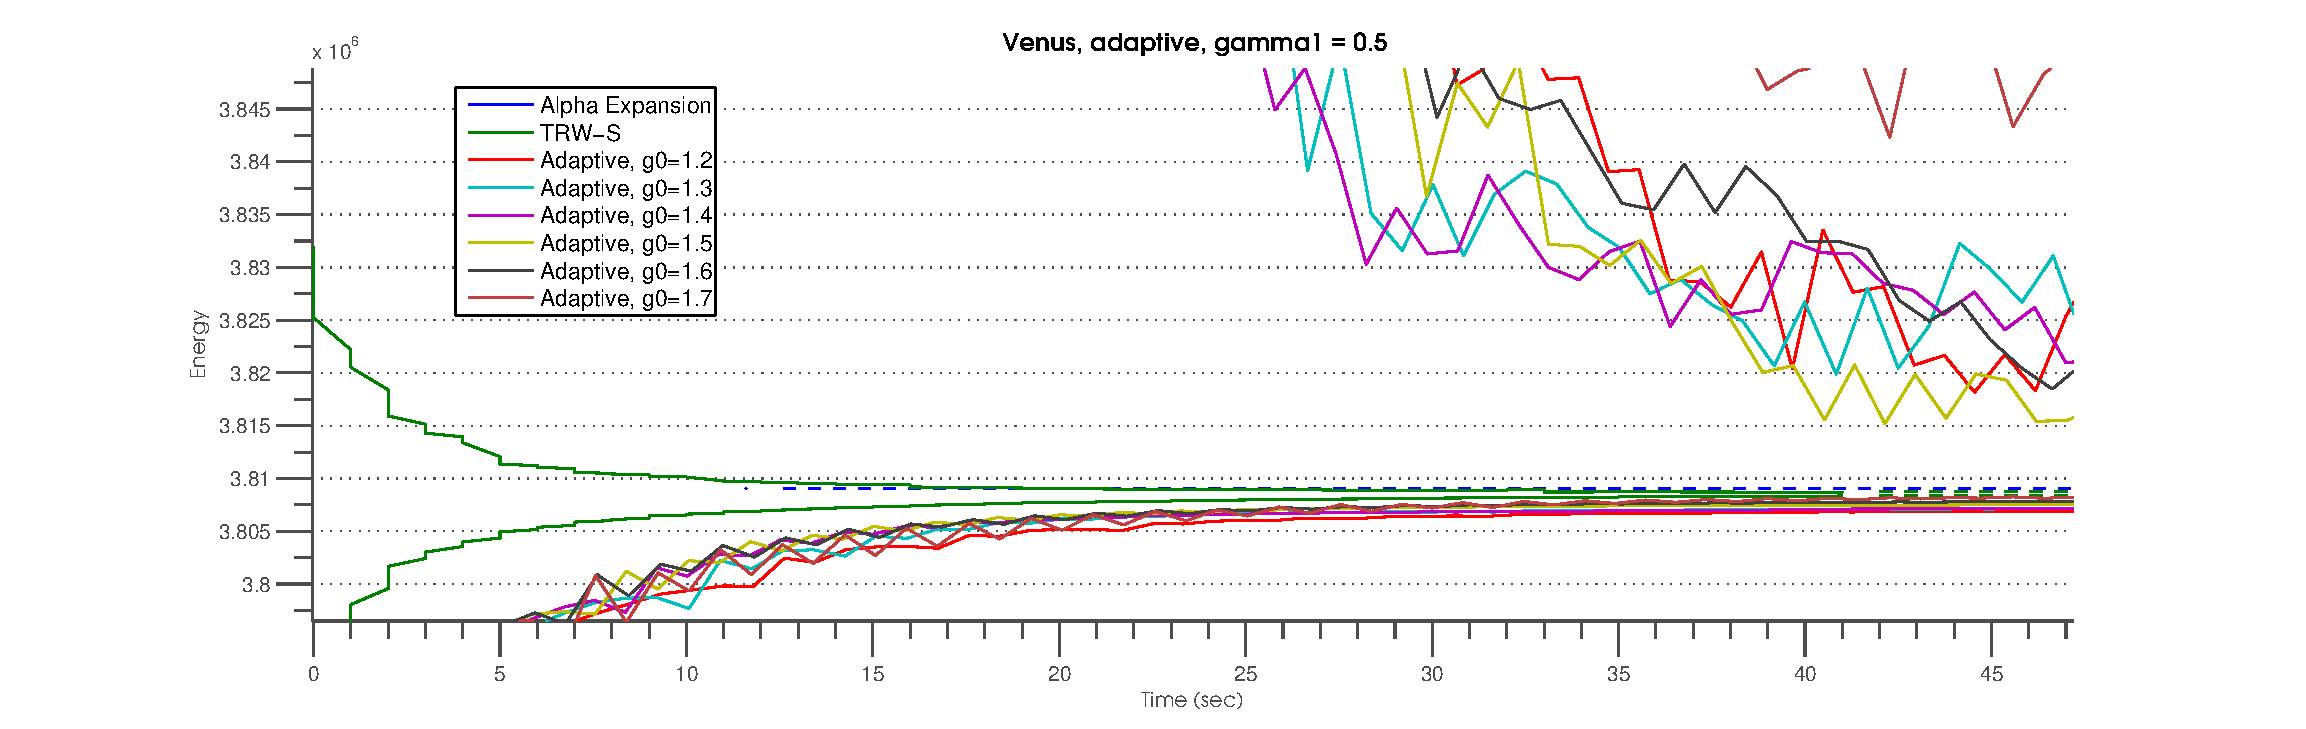
\includegraphics[width=\textwidth]{adaptive_g0_venus}
            \caption{Стерео--пара venus.}
    \end{subfigure}
    \begin{subfigure}[t]{\textwidth}
            \centering
            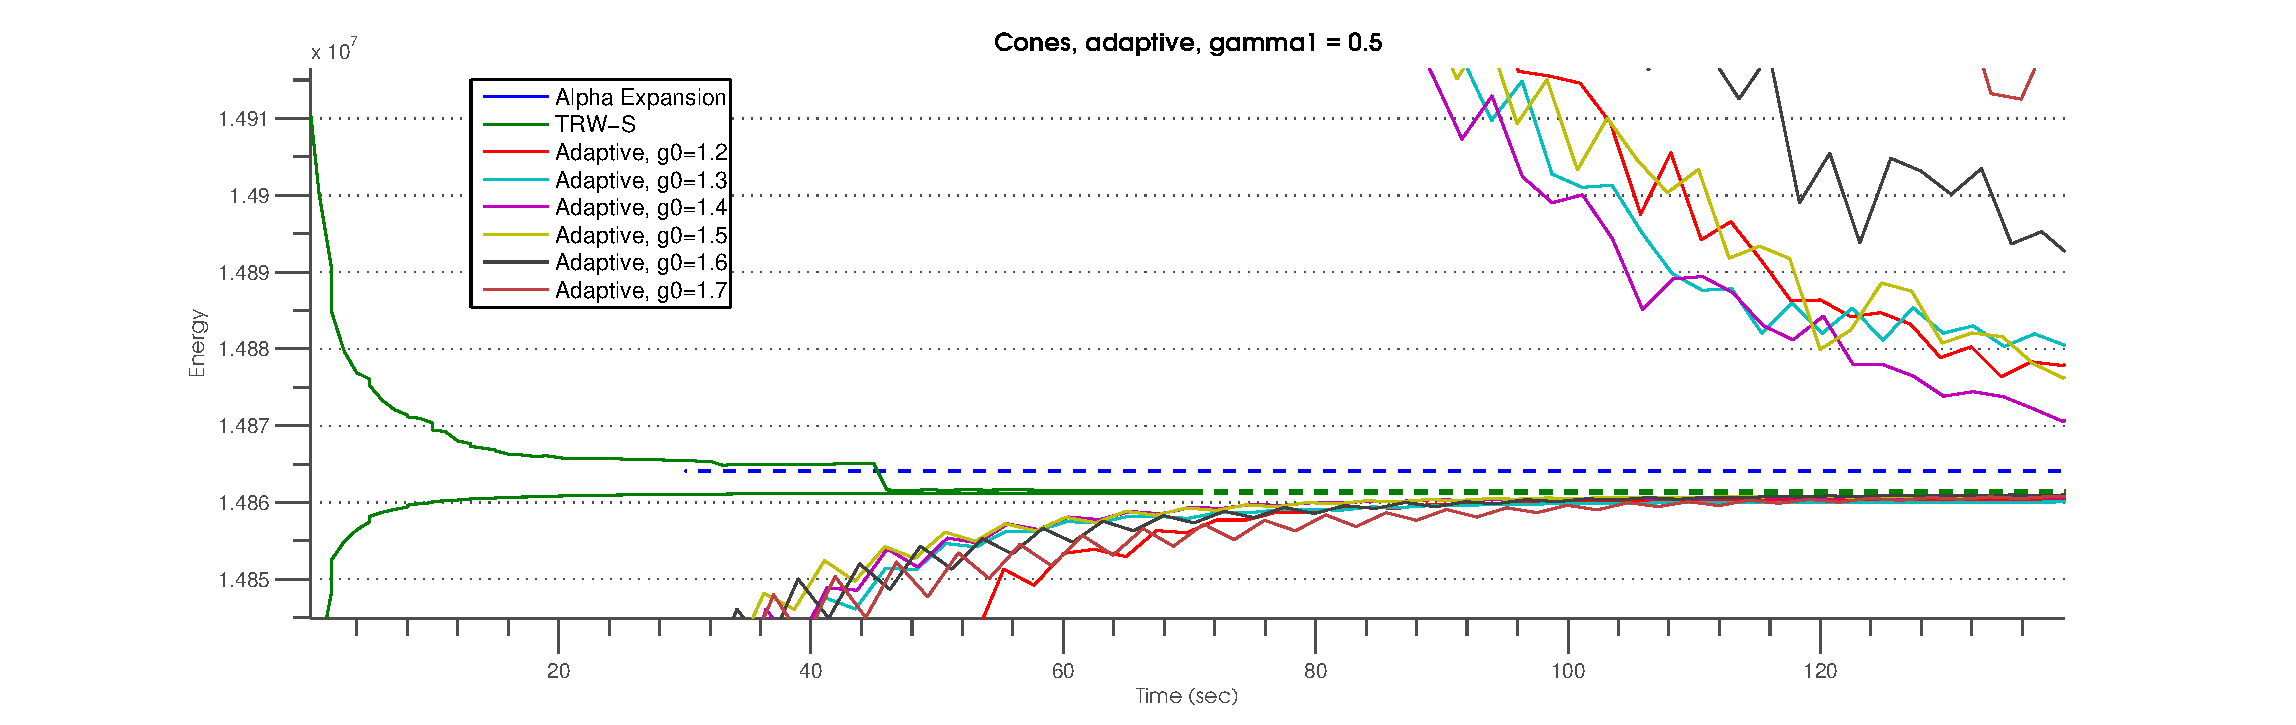
\includegraphics[width=\textwidth]{adaptive_g0_cones}
            \caption{Стерео--пара cones.}
    \end{subfigure}
    \begin{subfigure}[t]{\textwidth}
            \centering
            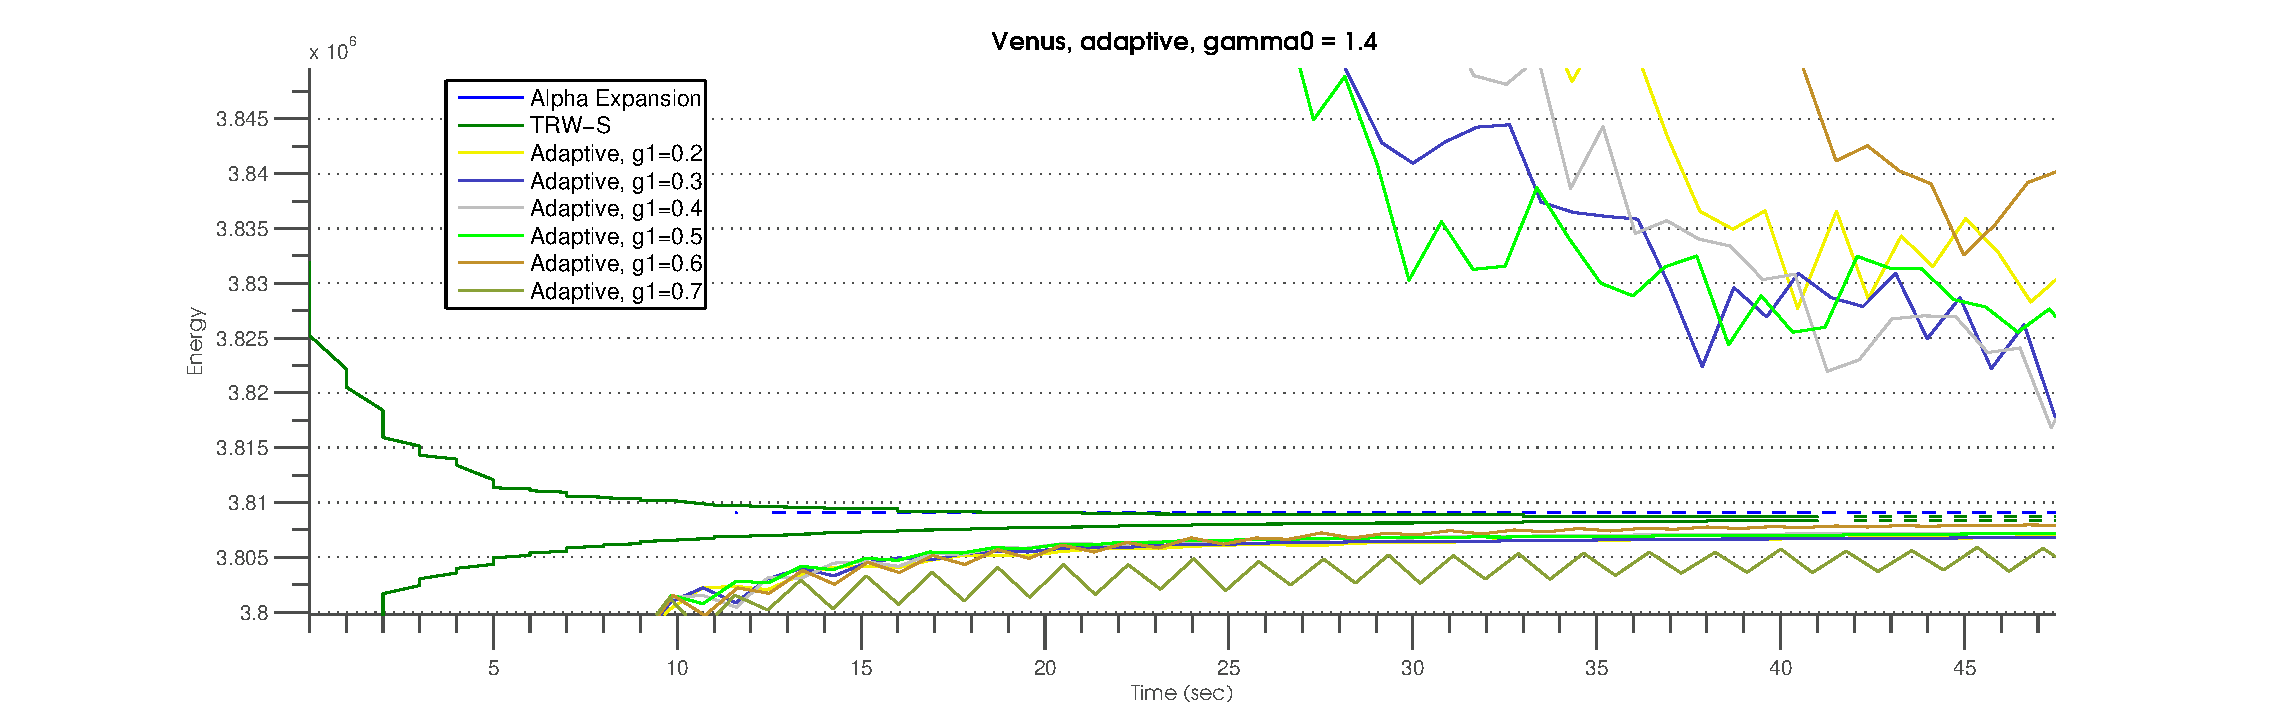
\includegraphics[width=\textwidth]{adaptive_g1_venus}
    \end{subfigure}
    \begin{subfigure}[t]{\textwidth}
            \centering
            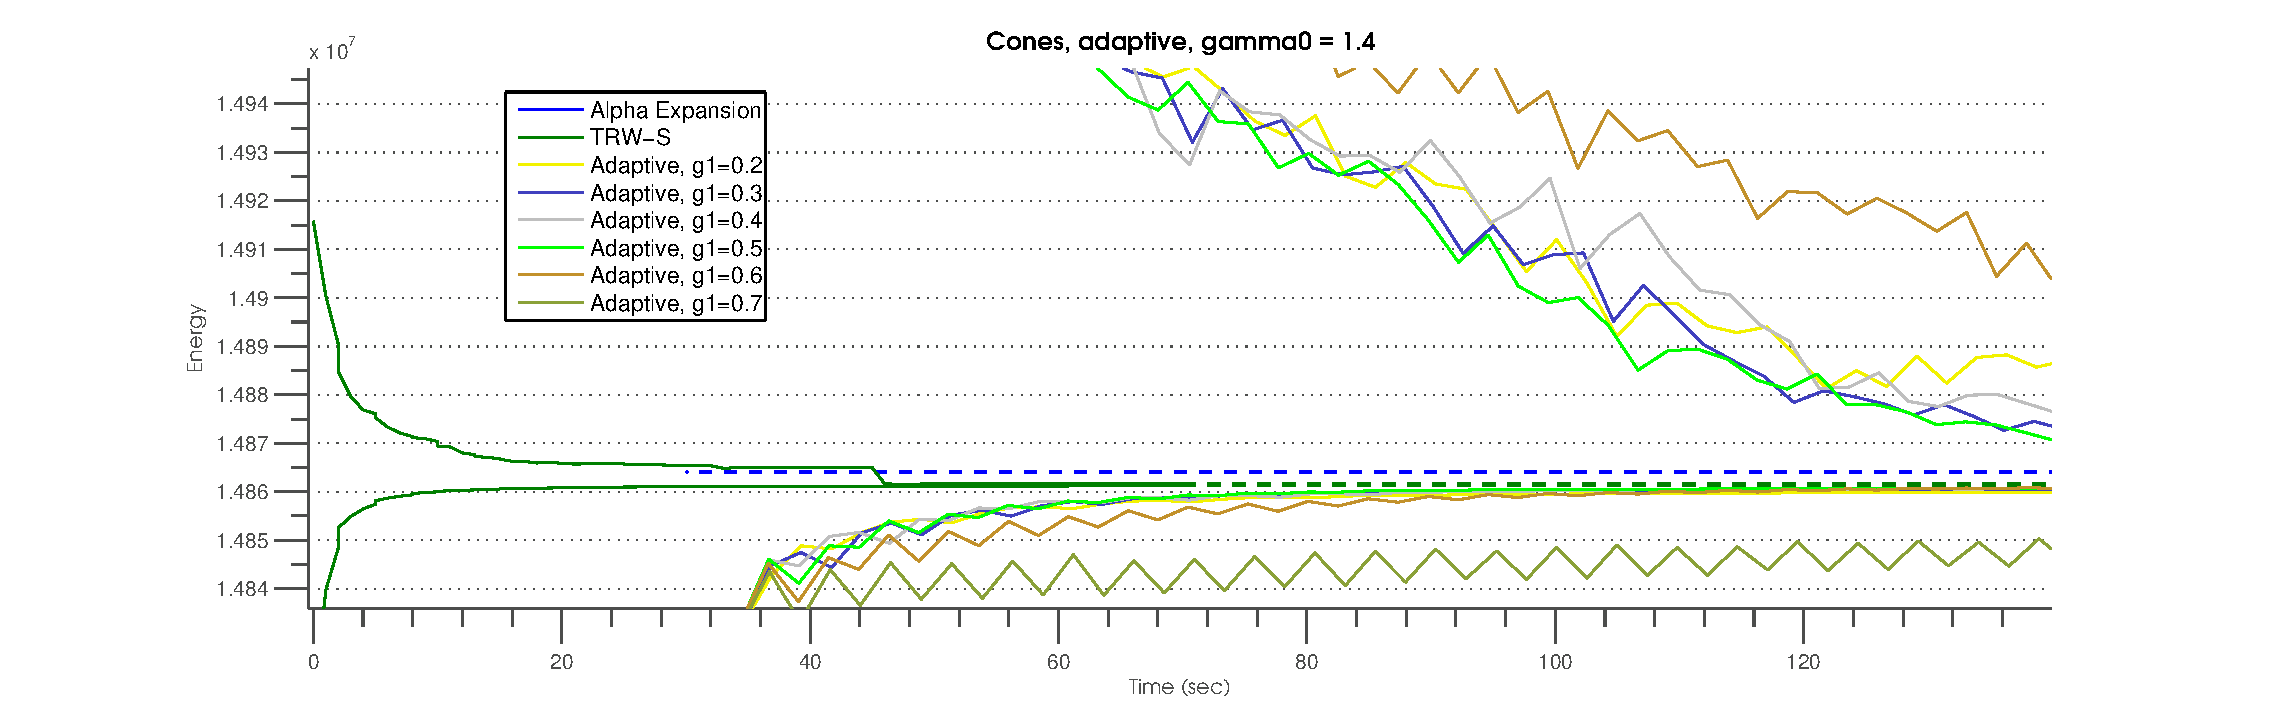
\includegraphics[width=\textwidth]{adaptive_g1_cones}
    \end{subfigure}
    \caption{Подбор параметров адаптивного субградиетного подъёма.}
    \label{fig:adaptive_params_extra}
\end{figure}

\begin{figure}
    \centering
    \begin{subfigure}[t]{\textwidth}
            \centering
            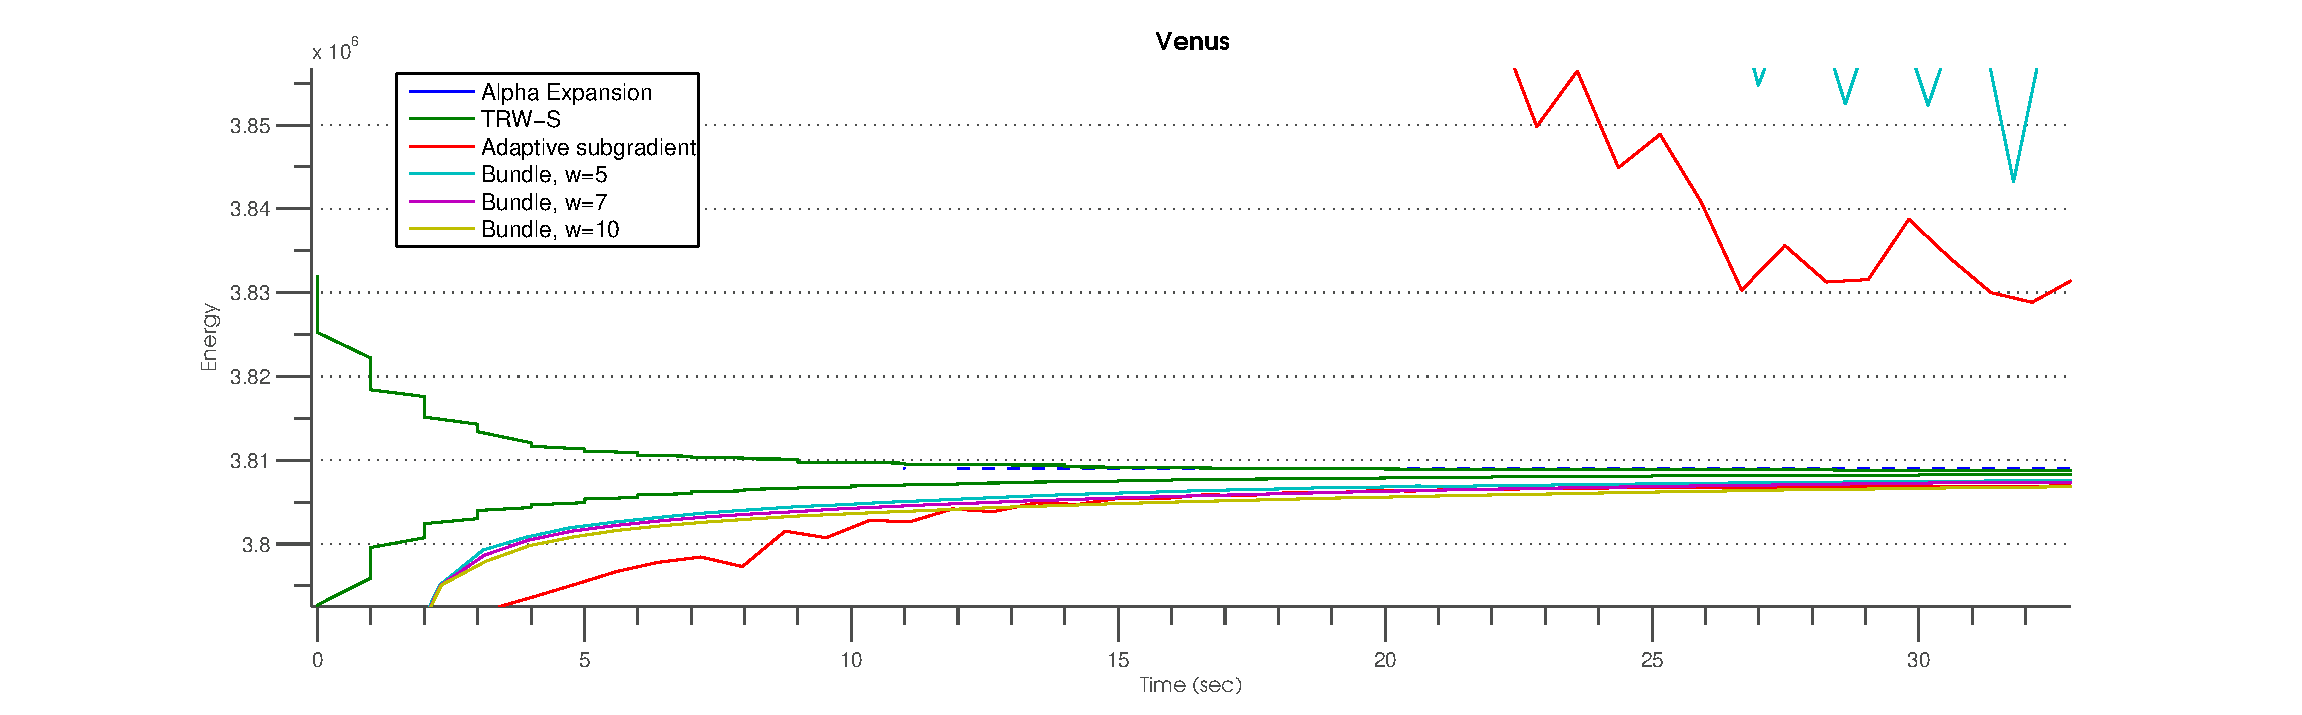
\includegraphics[width=\textwidth]{bundle_const_weight_venus}
    \end{subfigure}
    \begin{subfigure}[t]{\textwidth}
            \centering
            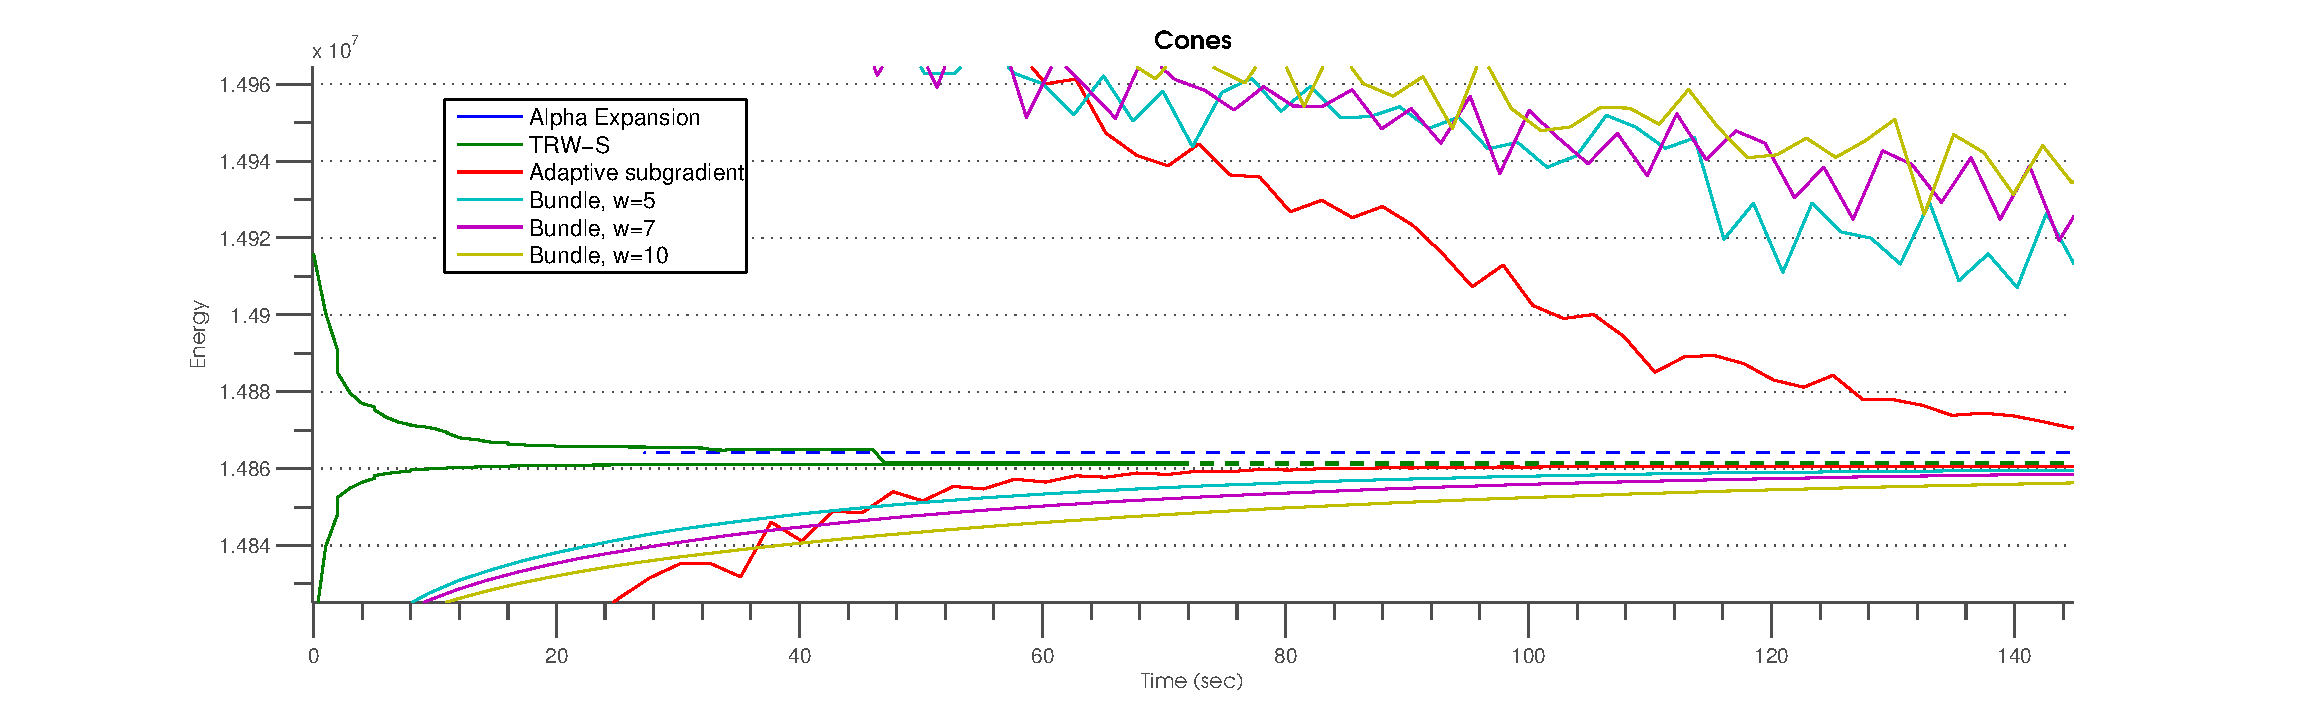
\includegraphics[width=\textwidth]{bundle_const_weight_cones}
    \end{subfigure}
    \caption{Метод пучка с различными константными весами.}
    \label{fig:bundle_const_weight_extra}
\end{figure}

\begin{figure}
    \centering
    \begin{subfigure}[t]{\textwidth}
            \centering
            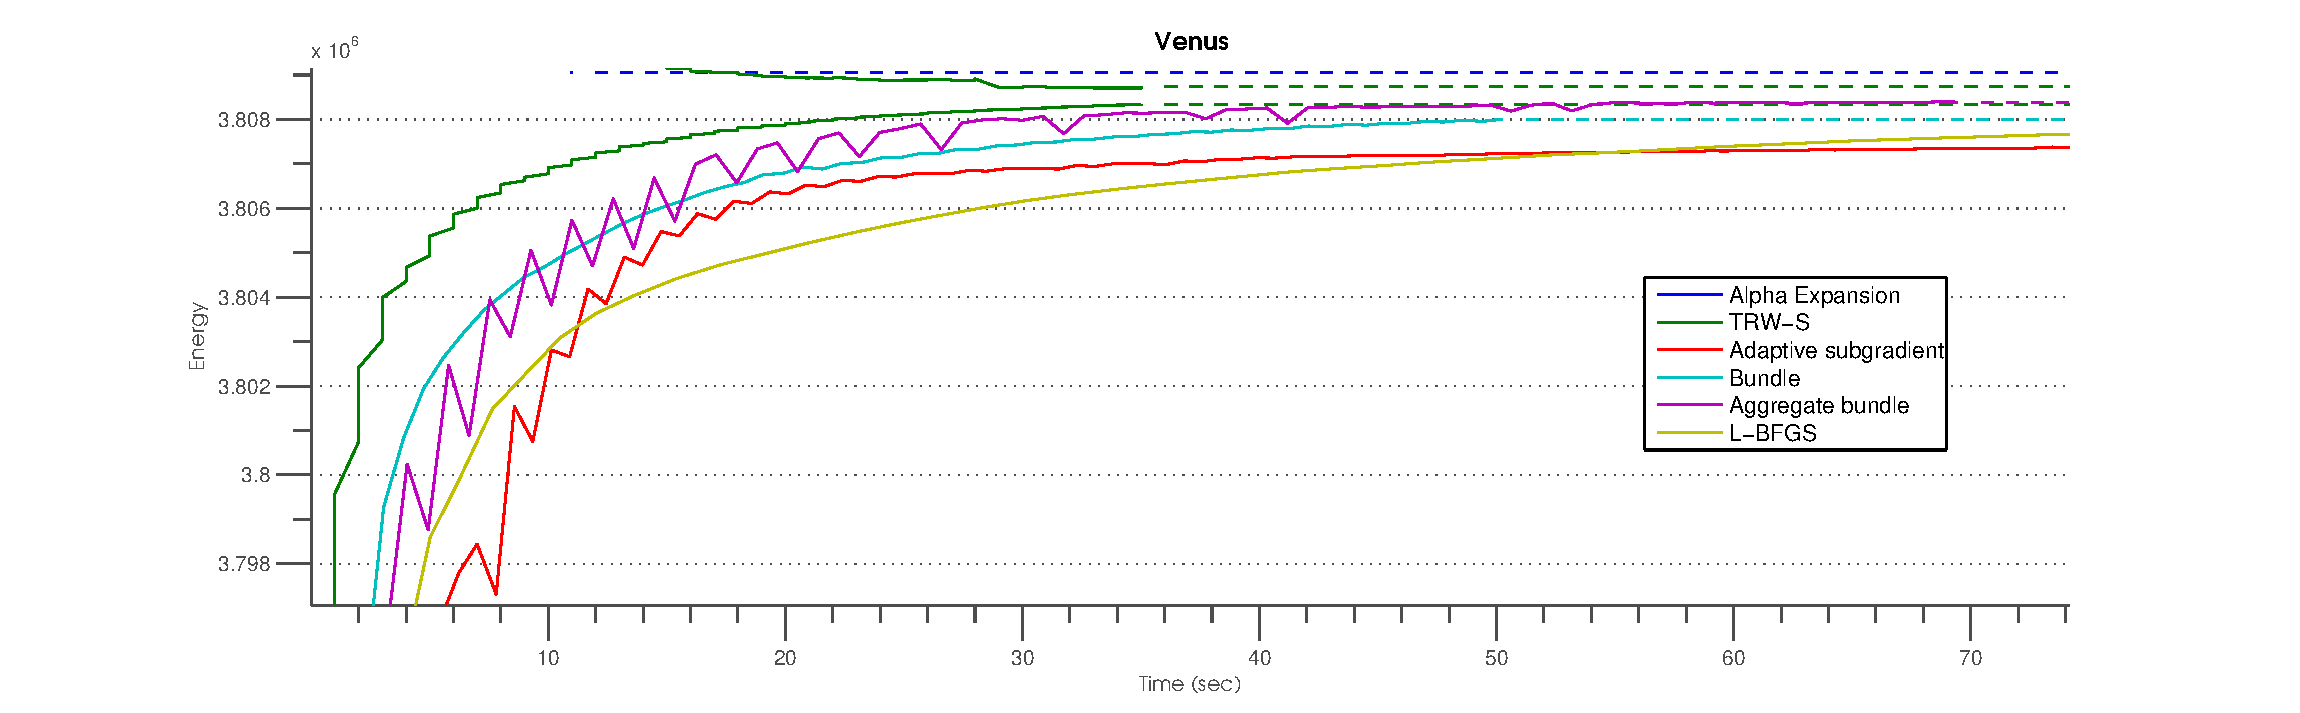
\includegraphics[width=0.9\textwidth]{comparative_venus.eps}
    \end{subfigure}
    \begin{subfigure}[t]{\textwidth}
            \centering
            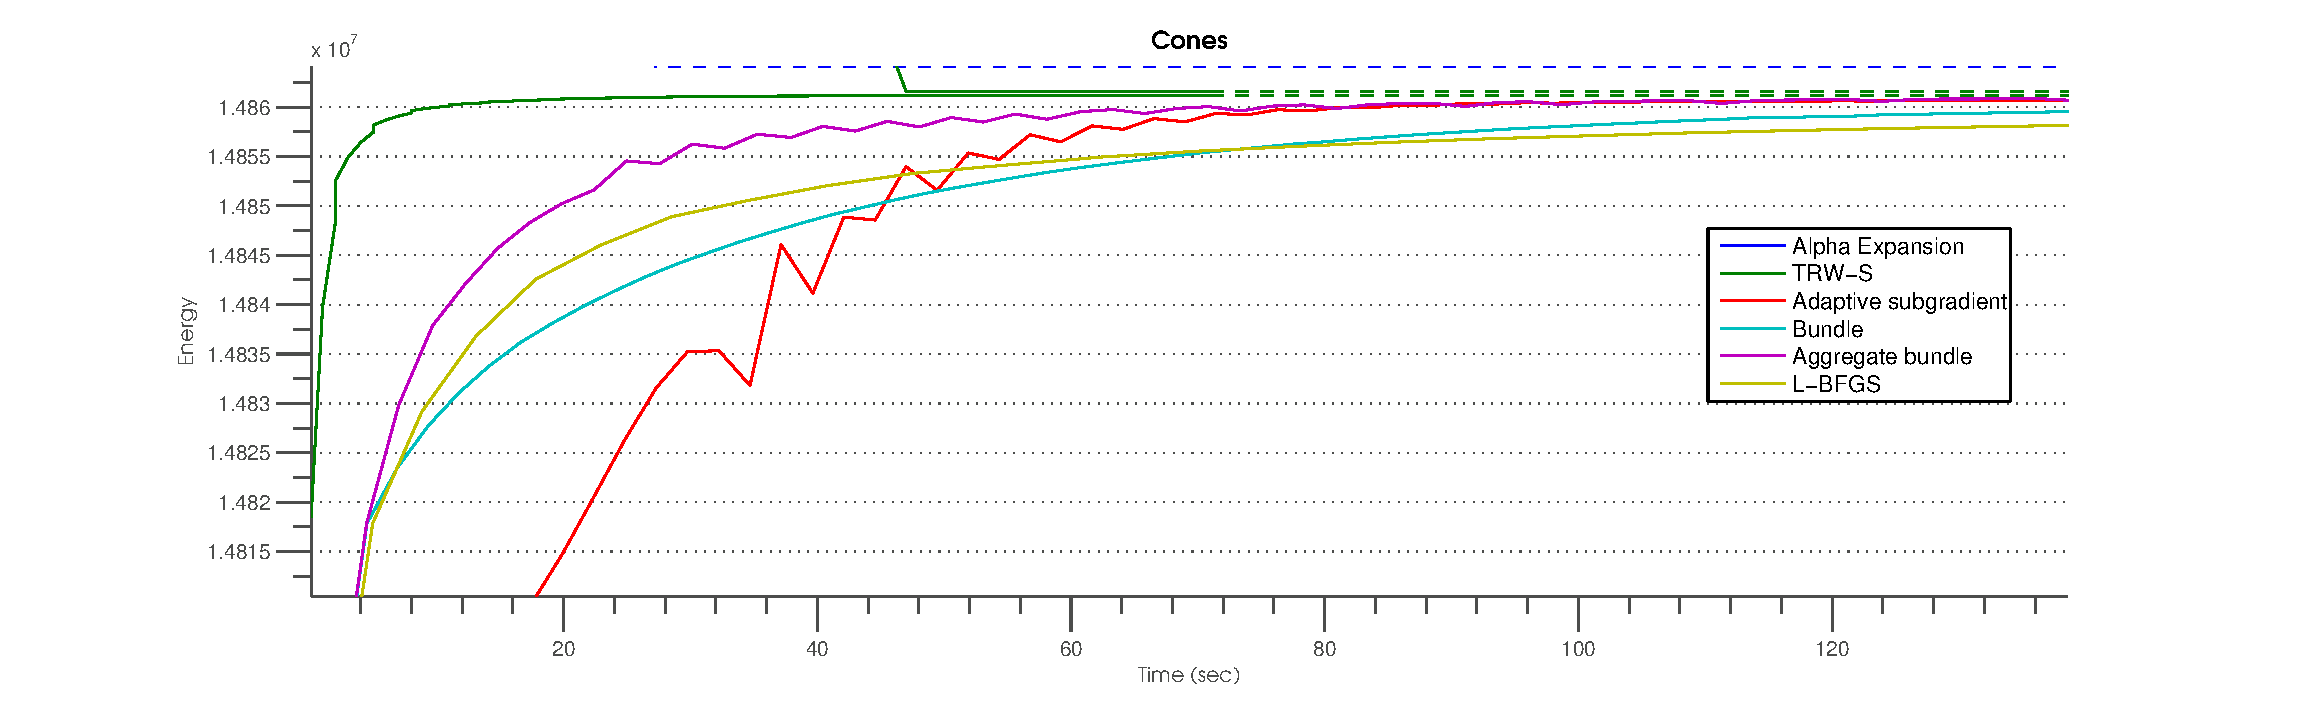
\includegraphics[width=0.9\textwidth]{comparative_cones.eps}
    \end{subfigure}
    \caption{Итоговое сравнение алгоритмов оптимизации энергии.}
    \label{fig:comparative_extra}
\end{figure}


\begin{thebibliography}{1}
\bibitem{AlphaExp}
    {Boykov~Y., Veksler~O., Zabih~R.}
    {Fast approximate energy minimization via graph cuts}~//
    {IEEE} Trans. Pattern Anal. Mach. Intell., 2001.~--- С.\,1222--1239.
\bibitem{ApplicationAndComp}
    {Szeliski~R.}
    {A comparative study of energy minimization methods for markov random fields with smoothness-based priors}~//
    {IEEE} Trans. Pattern Anal. Mach. Intell., 2008.~--- С.\,1068--1080.
\bibitem{AlphaExp2}
    {Kolmogorov~V., Zabin~R.}
    {What Energy Functions can be Minimized via Graph Cuts?}~//
    {IEEE} Trans. Pattern Anal. Mach. Intell., be.~--- С.\,147--159.
\bibitem{AlphaExp3}
    {Boykov~Y., Kolmogorov~V.}
    {An experimental comparison of min-cut/max-flow algorithms for energy minimization in vision}~//
    {IEEE} Trans. Pattern Anal. Mach. Intell., 2004.~--- С.\,1124--1137.
\bibitem{NewComparison}
    {Jörg~H.~K., Bjoern~A., Fred~A.~H.}
    {A Comparative Study of Modern Inference Techniques for Discrete Energy Minimization Problems}~//
    CVPR 2013
\bibitem{SubgradientWeights}
    {Komodakis~N., Paragios~N., Tziritas~G.}
    {MRF energy minimization and beyond via dual decomposition}~//
    {IEEE} Trans. Pattern Anal. Mach. Intell., 2011.~--- С.\,531--552.
\bibitem{belief_propagation}
    {Sun~J., Zheng~N.~N., Shum~H.~Y.}
    {Stereo matching using belief propagation}~//
    {IEEE} Pattern Analysis and Machine Intelligence, 2003.~--- С.\,787--800.
\bibitem{TRWS}
    {Kolmogorov~V.}
    {Convergent Tree-Reweighted Message Passing for Energy Minimization}~//
    {IEEE} Trans. Pattern Anal. Mach. Intell., 2006.~--- С.\,1568--1583.
\bibitem{ABundle}
    {Kiwiel~K.}
    {An aggregate subgradient method for nonsmooth convex minimization}~//
    Mathematical Programming, 1983, 27:320--341.
\bibitem{Alahari}
    {Alahari~K., Kohli~P., Torr~P.~H.~S.}
    {Dynamic Hybrid Algorithms for MAP Inference in Discrete MRFs}~//
    {IEEE} Trans. Pattern Anal. Mach. Intell., 2010.~--- С.\,1846--1857.
\bibitem{Subgradient}
    {Komodakis~N., Paragios~N., Tziritas~G.}
    {MRF energy minimization and beyond via dual decomposition}~//
    Pattern Analysis and Machine Intelligence, IEEE Transactions on, 2011.~--- С.\,531--552.
\bibitem{Bundle}
    {Kappes~J.\,H., Bogdan~Savchynskyy, Christoph~Schnorr}
    {A Bundle Approach To Efficient MAP-Inference by Lagrangian Relaxation}~//
    Computer Vision and Pattern Recognition (CVPR), IEEE Conference 2012.~--- С.\,1688--1695.
\bibitem{Bundle}
    {Kappes~J.\,H., Bogdan~Savchynskyy, Christoph~Schnorr}
    {A Bundle Approach To Efficient MAP-Inference by Lagrangian Relaxation}~//
    Computer Vision and Pattern Recognition (CVPR), IEEE Conference 2012.~--- С.\,1688--1695.
\bibitem{1d_optimization}
    \small\url{http://www.machinelearning.ru/wiki/images/a/a8/MOMO12_min1d.pdf}~---
    Кропотов~Д.~А., Методы одномерной минимизации, 2012.
\end{thebibliography}
\end{document}

